\documentclass[letterpaper, 12pt]{article}

\usepackage[english]{babel}
\usepackage[margin=0.85in]{geometry}
\usepackage{graphicx}
\usepackage{float}
\usepackage{subcaption}
\PassOptionsToPackage{hyphens}{url}\usepackage{hyperref}
\newenvironment{allintypewriter}{\ttfamily}{\par}
\hypersetup{
  colorlinks,
  citecolor=black,
  filecolor=black,
  linkcolor=black,
  urlcolor=blue
}

\def\bsq#1{%both single quotes
	\lq{#1}\rq}

\usepackage{listings}
\usepackage{color}

\definecolor{dkgreen}{rgb}{0,0.6,0}
\definecolor{gray}{rgb}{0.5,0.5,0.5}
\definecolor{mauve}{rgb}{0.58,0,0.82}

\lstset{frame=tb,
	language=Java,
	aboveskip=3mm,
	belowskip=3mm,
	showstringspaces=false,
	columns=flexible,
	basicstyle={\small\ttfamily},
	numbers=none,
	numberstyle=\tiny\color{gray},
	keywordstyle=\color{blue},
	commentstyle=\color{dkgreen},
	stringstyle=\color{mauve},
	breaklines=true,
	breakatwhitespace=true,
	tabsize=3
}

\graphicspath{{pictures/}}
\newcommand\TSAT{\textbf{TSAT}}

\begin{document}
\title{User Manual: Using RPM with TSAT}
\maketitle
\tableofcontents
\newpage

\section{Introduction to TSAT}


{\TSAT} or the Time Series Analysis Tool is a software application that has enhanced the capabilities of GrammarViz 2.0 and 3.0~\cite{senin-anomaly,senin-gv2,senin-gv3}.  {\TSAT} has three main features:
\begin{description}
	\item[Supervised Classification] Using labeled time series train an algorithm to classify unknown time series
	\item[Motif Discovery] Finding repeated patterns within a time series
	\item[Anomaly Detection] Finding rarely repeated patterns within a time series
\end{description}

\subsection{Interface Layout}
The main method for interacting with {\TSAT} in this user guide will be through the graphical user interface, or the GUI.  When TSAT is started the GUI should look like that in Figure~\ref{fig:tsat-interface}.

\begin{figure}[H]
	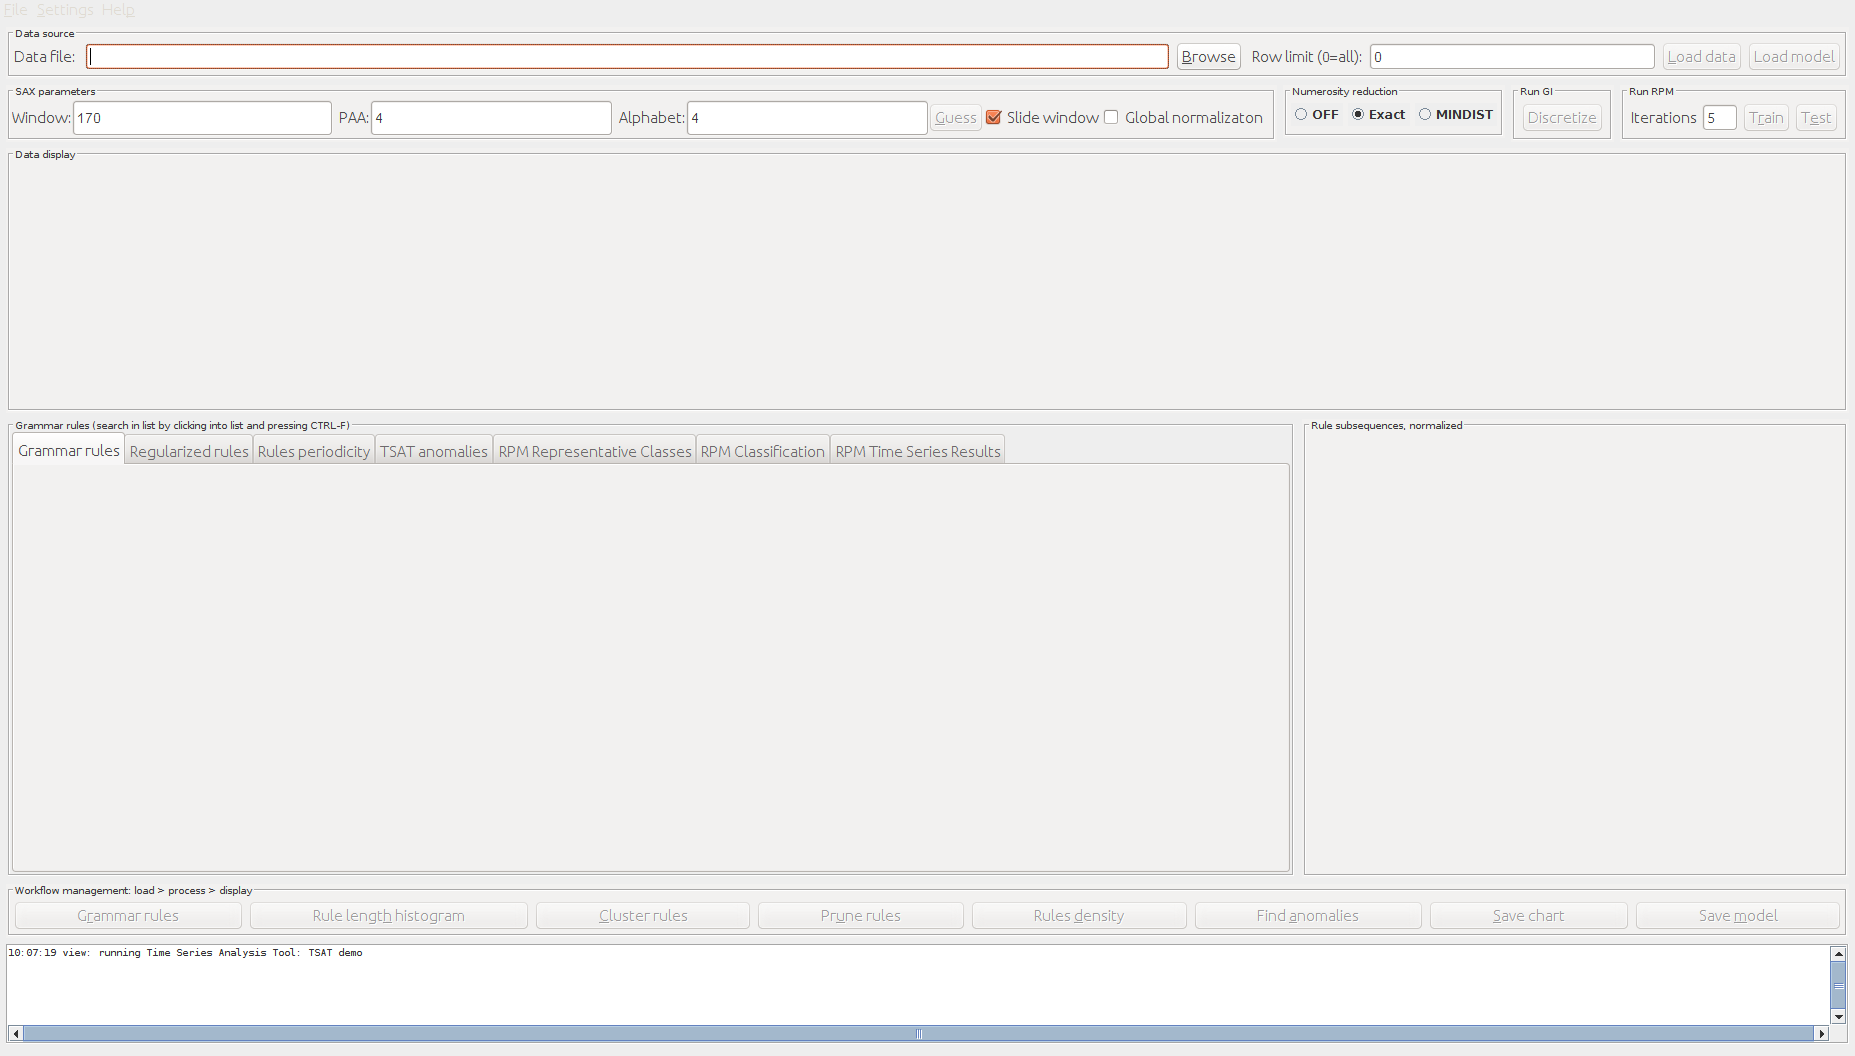
\includegraphics[width=\textwidth]{pictures/TSAT-interface}
	\caption{Initial state of the {\TSAT} Graphical User Interface (GUI).}
	\label{fig:tsat-interface}
\end{figure}

There are eleven regions in the main GUI used to set parameters, load files, and analyze results.  The nine main regions in the GUI have a rectangular outline around them with a label.  They include: ``Data Source'', ``SAX Parameters'', ``Numerosity reduction'', ``Run GI'', ``Run RPM'', ``Data display'', ``Grammar rules'', ``Rule Subsequences, normalized'', and ``Workflow management.''  The other two regions are the top menu bar (with ``File'', ``Settings'', and ``Help'') and the text area at the bottom of the GUI.  Presently, the items under ``Help'' do not have any meaningful functionality.  The text area at the bottom of the GUI is used to log useful information about the state of GUI.  That text area may also be referred to as the logging area.

\subsection{Python Interface}
In addition to a Graphical User Interface, {\TSAT} also has a python interface.  This interface consists of wrappers of the major functionality of {\TSAT}'s GUI. 

The python interface is found in the python directory as python/tsail.py.  In order for the python interface to work, the {\TSAT} jar must be located in:\\ \texttt{/target/tsat-0.0.1-SNAPSHOT-jar-with-dependencies.jar}\\
If it is not there, either its alternative location must be set within tsail.py by editing within tsail.py the following variable to the correct location:
\begin{lstlisting}
TSAT_JAR_LOCATION = "../target/tsat-0.0.1-SNAPSHOT-jar-with-dependencies.jar"
\end{lstlisting} 
or {\TSAT} can be recompiled by running:\\
\noindent\texttt{mvn package -Psingle}\\
which will generate the jar file in the correct location:\\
\texttt{/target/tsat-0.0.1-SNAPSHOT-jar-with-dependencies.jar}\\
In the python directory in TSAT you can run python and then type:
\begin{lstlisting}
import tsail
\end{lstlisting}

Then you can call the functions like
\begin{lstlisting}
tsail.buildMotifs(pathToTimeseries, outputFile, window_size=30, word_size=6, alphabet_size=4, strategy="EXACT", threshold=0.01, numworkers=2)
tsail.RRA(pathToTimeseries, outputFile, window_size=30, word_size=6, alphabet_size=4, threshold=0.01, discords_num=5)
tsail.RPMTrainTest(pathToTraining, pathToTest, outputFile, num_iters)
tsail.RPMTrain(pathToTraining, outputFile, num_iters)
tsail.RPMTest(pathToTest, modelFile, num_iters)
\end{lstlisting}

For motifs, anomaly detection and representative pattern matching respectively.  In each of the chapters on Motif Discovery, Anomaly detection, and Time Series Classification there are instructions on how to use these functions.  Examples of their usage are also provided within tsail.py.

\subsection{Tools Introduction}
{\TSAT} provides implementations of a number of algorithms used to analyze time series including Representative Pattern Mining (RPM) to perform time series classification, Motif Discovery to find repeating patterns, and Discord Discovery to detect anomalies.


\subsubsection{Motif Discovery}
\label{MotifSec}
A motif is a reoccurring pattern within a time series (an example motif is shown in Figure~\ref{fig:tsat-example-motif}) and both anomaly detection and representative pattern mining build from this concept.  In order to identify motifs within a time series {\TSAT} first converts the time series into a string (a sequence of words) and then performs context free grammar induction (GI).  Specifically {\TSAT} executes two main algorithms SAX (Symbolic Aggregate Approximation) with numerosity reduction and a user chosen GI algorithm either Sequitur or Re-Pair~\cite{senin-gv2,nevill1997identifying,larsson2000off}.  The motifs are then defined as the subsequences in the time series defined by the grammar rules.  {\TSAT} allows the user to explore the motifs by sorting by how frequently the rule is used in the root rule (labeled R0 in {\TSAT}).

\paragraph{SAX}SAX converts the time series into a string, or a sequence of characters.  It does this by using a fixed size sliding window over the time series and performing Piecewise Aggregate Approximation (PAA) on each window and converting those values into words.  This is called subsequence discretization~\cite{lonardi2002finding}.

First SAX splits the time series up into smaller time series by only looking at a fixed size window, or subsequence extraction as seen in Figure~\ref{fig:tsat-slidingwindow}.  So, if the time series is of length 1000 and the window length is 100 then each time series that SAX looks at is of length 100.  SAX uses a sliding window with a step size of one.  This means that the first time series given the same example spans from timestep 1 to 100 and the second time series is 2 to 101 and so there will be 999 different time series of length 100.  The formula is \(n - w + 1\) where \(n\) is the length of the time series and \(w\) is the length of the sliding window (the \textbf{window length}).

\begin{figure}[H]
	\centering
	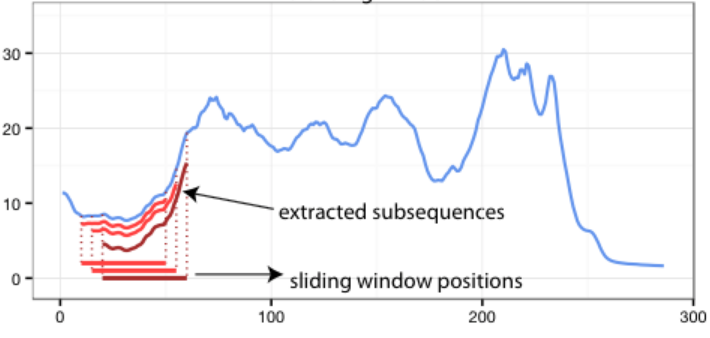
\includegraphics[width=0.7\textwidth]{pictures/TSAT-slidingwindow}
	\caption{Subsequence extraction from a sliding window.  Adopted from:\\ \url{http://grammarviz2.github.io/grammarviz2_site/morea/assets/sax-error.png}}
	\label{fig:tsat-slidingwindow}
\end{figure}


Then for each sliding window time series, PAA produces a word by first performing z-normalization on the values.  This means converting the time series values to values with a mean and standard deviate of approximately 0 and 1 respectively.  However, so as to not amplify the ``under-threshold-noise'' there is a \textbf{z-normalization threshold} value so that if the input time series' standard deviation is less than this value the z-normalization will not be applied. Then the algorithm splits the window up into \(m\) equal sized segments called the \textbf{PAA size} and for each of the segments it computes the mean value.  

SAX maps each mean value to a letter in the alphabet and produces a word (a sequence of letters/characters).  The number of characters, \(a\), available in the alphabet is chosen by the user (the \textbf{alphabet size}).  Since the values of z-normalized time series follow the Normal distribution~\cite{lin2003symbolic}, the breakpoints for each character can be determined by making \(a\) equal-sized areas under the Normal curve using lookup tables (illustrated along the y-axis in Figure~\ref{fig:tsat-sax}). Then for each of the windows we have created a word.  Figure~\ref{fig:tsat-sax} shows the process of converting a time series (without any sliding window) into a SAX word.  It should be pointed out that the ``observation that normalized subsequences have highly Gaussian distribution, is not critical to correctness of any of the algorithms that use SAX, including the ones in this work. A pathological dataset that violates this assumption will only affect the efficiency of the algorithms''~\cite{keogh2004hot}.

\begin{figure}[H]
	\centering
	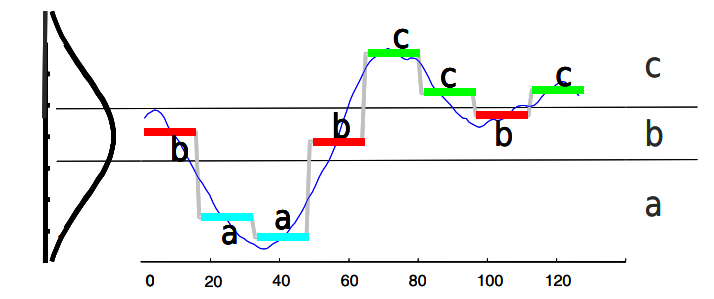
\includegraphics[width=.7\textwidth]{pictures/TSAT-SAX}
	\caption{``A time series is discretized by first obtaining a PAA approximation and then using predetermined breakpoints to map the PAA coefficients into SAX symbols. In the example above, with n = 128, w = 8 and a = 3, the time series is mapped to the word baabccbc.''  Both the figure and the included caption are from~\cite{lin2007experiencing}.}
	\label{fig:tsat-sax}
\end{figure}


\paragraph{Numerosity Reduction}The list of words produced using this procedure is also compressed using numerosity reduction.  Numerosity reduction reduces the size of this list of words by skipping duplicate words.  Additionally, ``numerosity reduction makes motif discovery more robust, as we are matching patterns based on their shapes, even if they do not have the exact same lengths''~\cite{li2012visualizing}.  For example, a time series \(S_{1}\) 

\[
S_{1}= aac_{1}\, aac_{2}\, abc_{3}\, abb_{4}\, acd_{5}\, aac_{6}\, aac_{7}\, aac_{8}\, abc_{9}\, \dots
\]
is converted to the much smaller string using numerosity reduction:
\[S2 = \textit{aac}_{1}~ \textit{abc}_{3}~ \textit{abb}_{4}~ \textit{acd}_{5}~ \textit{aac}_{6}~ \textit{abc}_{9}\]
where the subscripts are the window numbers.

\paragraph{Grammar Induction GI}Then grammar induction is used to produce grammar rules, the motifs, from the SAX string. Both Sequitur and Re-Pair are context free grammar induction algorithms that are included in {\TSAT}.  {\TSAT} uses Sequitur as its default.  However, there are a number of differences according to~\cite{readmeGI}:
\begin{itemize}
	\item Sequitur implementation is slower than Re-Pair
	\item Sequitur tends to produce more rules, but Sequitur rules are less frequent than Re-Pair rules
	\item Sequitur rule-corresponding subsequences vary in length more
	\item Sequitur rules usually cover more points than Re-Pair
	\item Sequitur rule coverage depth is lower than that of Re-Pair
\end{itemize}

A simple example (not a time series) of a context free grammar is to take the following string ``a rose is a rose is a rose'' this can be converted to the following grammar rules:

\begin{center}
	S \(\rightarrow\) BBA\\
	A \(\rightarrow\) B is\\
	B \(\rightarrow\) a rose\\
\end{center}
Where S is the root rule, meaning that no rule uses this rule and A and B are grammar rules that are used in S. Also, note that the grammar forms a hierarchy and therefore will not contain cycles.  As the above example illustrates the lengths of the motifs can be of varying lengths as the rule may contain other rules (note that in an actual time series each word would be the same length).
\begin{figure}[H]
	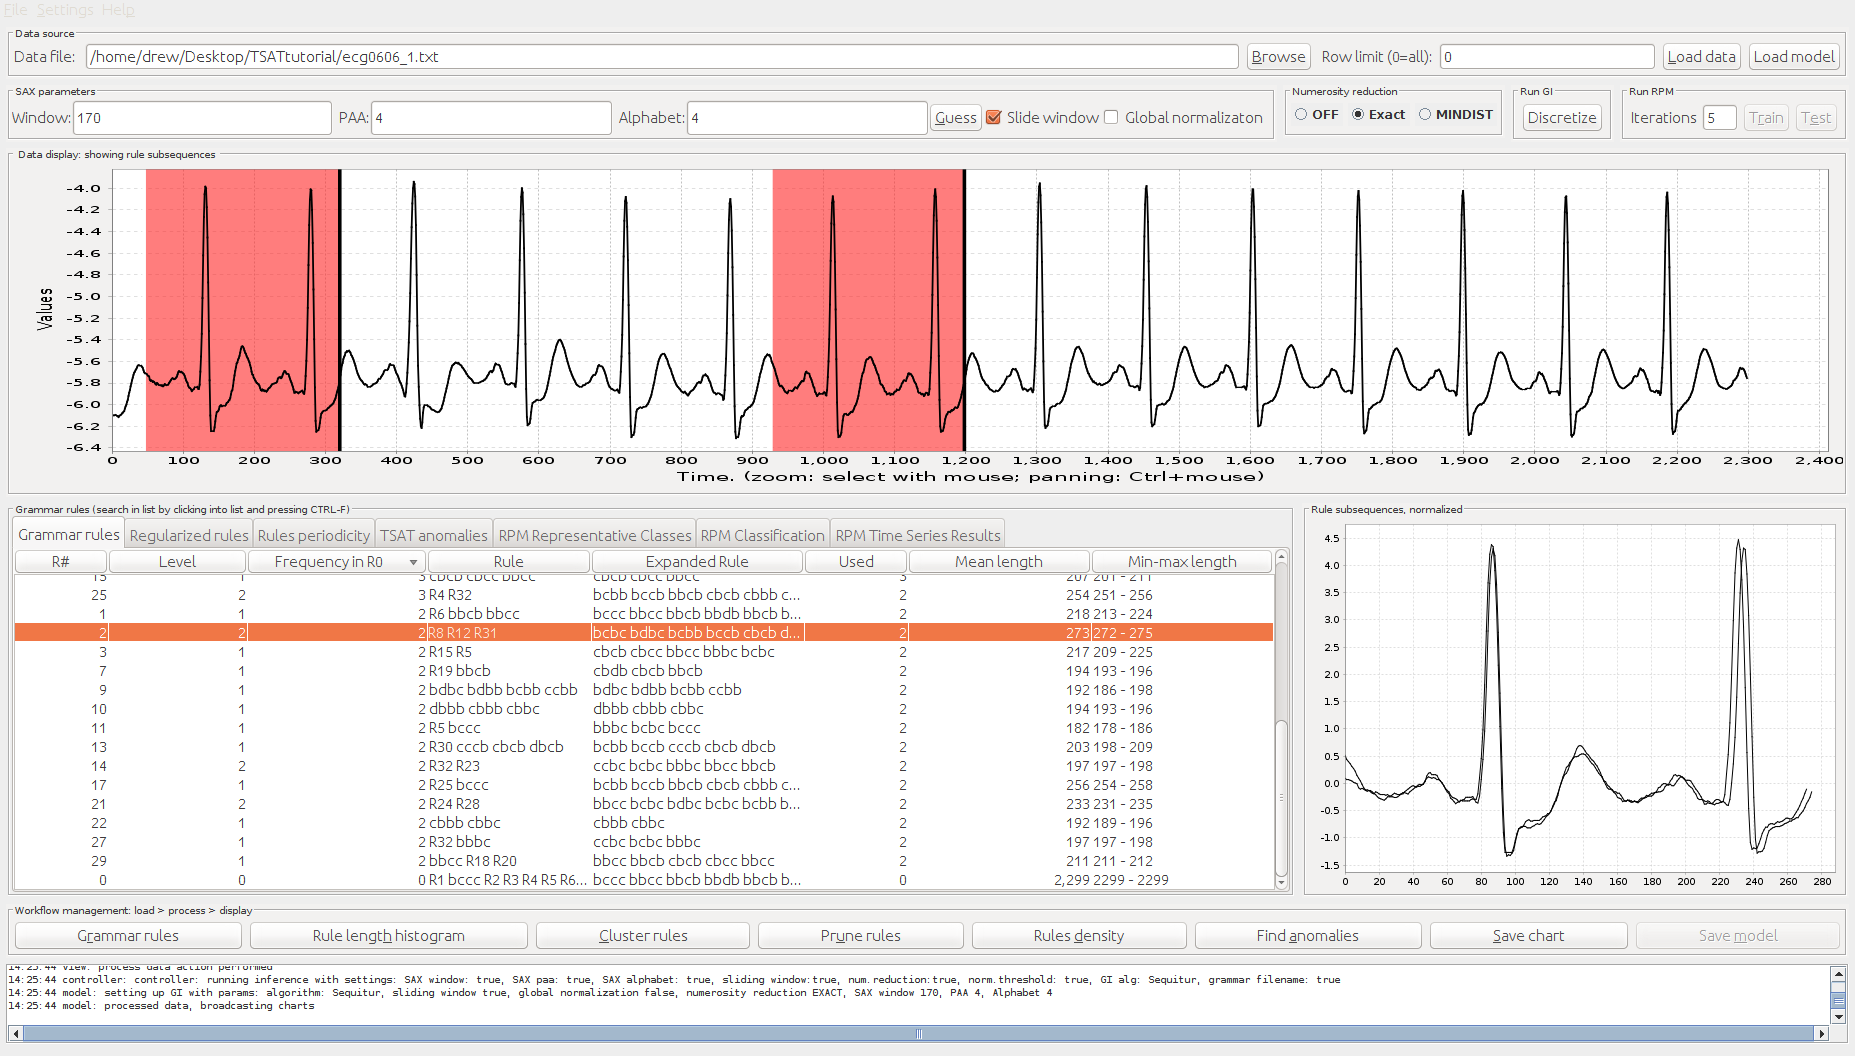
\includegraphics[width=\textwidth]{pictures/TSAT-example-motif}
	\caption{Example motif found using {\TSAT} with the subsequences highlighted in the Data Display and shown in the Rules Subsequences areas.}
	\label{fig:tsat-example-motif}
\end{figure}
\paragraph{Setting the Parameters}One example motif found by {\TSAT} in ECG data is shown in Figure~\ref{fig:tsat-example-motif}.  There are only three parameters, alphabet size, PAA length, and window size.  Past studies have empirically shown that an alphabet size of 3 or 4 will work in most settings and that the PAA length depends on the data.  The PAA length (also known as word size) tends to be a smaller value for smooth and slow changing time series and a larger value for more complex time series~\cite{keogh2004hot}. ``Note however, that grammar induction step effectively mitigates improper sliding window selection''~\cite{motifSite}.


\subsubsection{Anomaly Detection}

%Anomalies are discords the subsequences whose distance to their nearest non-self match is the largest.

%anomalous subsequences correspond to rare grammar rules, we call the algorithm RRA (Rare Rule Anomaly)

%A subsequence is a non-self match with another subsequence if there subsequences do not overlap

{\TSAT} also implements two anomaly detection algorithms taking an exact approach and an approximate approach~\cite{senin2015time}.  Specifically the \textbf{Rare Rule Anomaly} (RRA) algorithm and the \textbf{rule density curve} algorithm.  Each method uses the grammar rules generated by Sequitur or Re-Pair to extract the corresponding subsequences in the time series.  However, each method uses these subsequences in a different way.

RRA defines anomalous subsequences as \textit{discords} or the subsequences whose euclidean distance (normalized by the subsequence length) to their nearest non-self match is the largest.  A subsequence is a non-self match with another subsequence if their subsequences do not overlap. 

The approximate anomaly detection method is implemented using the rule density curve.  The value at each point in the rule density curve is the number of grammar rules that span or ``cover'' the corresponding point in the time series.  Therefore, ``rule density curve intervals that contain minimal values correspond to time series anomalies''~\cite{senin2015time}.  

Both the exact and approximate methods can find variable length anomalies.  However, ``if the time series under analysis has low regularity (an issue that impacts the grammar’s hierarchy) or the discretization parameters are far from optimal and regularities are not conveyed into the discretized space, the rule density based anomaly discovery technique may fail to output true anomalies''~\cite{senin2015time}.  Therefore, using the exact approach is preferable.
\paragraph{Setting the Parameters} The best advice is from~\cite{senin2015time}:

\begin{quote}
	Specifically, we found that the rule density curve facilitates the discovery of patterns that are much shorter than the window size, whereas the RRA algorithm naturally enables the discovery of longer patterns. Second, we observed that when the selection of discretization parameters is driven by the context, such as using the length of a heartbeat in ECG data, a weekly duration in power consumption data, or an observed phenomenon cycle length in telemetry, sensible results are usually produced.
\end{quote}


\subsubsection{Representative Pattern Mining - RPM}
\label{RPMOverview}



Univariate multiclass supervised time series classification is implemented in {\TSAT} with \textbf{Representative Pattern Mining} or \textbf{RPM}~\cite{wang2016rpm}.  RPM works by identifying an optimal sliding window size, PAA size, and alphabet length for each class and it identifies the motifs that match the class it belongs to more so than the other classes.  RPM then refines the set of motifs to the most representative and uses them to perform time series classification.

Here are some definitions to a few common machine learning terms that you may encounter:

\begin{description}
	\item[Attribute] An attribute, variable, or feature is a value that is used to describe the data point.  For example, a time series is an attribute.
	\item[Class] A class or label is the name used to describe a set of attributes.  In classification the goal is to classify examples as belonging to a particular class or to assign a label.
	\item[Example] An example is the set of attributes used to describe a single data point.
	\item[Univariate] Univariate, single attribute, or single feature means that each example is represented by a single attribute.  This means a single time series in time series classification is defined to be an example.
	\item[Multivariate] Multivariate, multi-attribute, or a feature vector means that each example is represented by multiple attributes.
	\item[Supervised Classifier] An algorithm that creates a model representation from a set of labeled examples in order to classify unlabeled examples.  Some example classification algorithms are, Support Vector Machine, Random Forest, Logistic Regression, AdaBoost, or Naive Bayes.
	\item[Training Data] The set of labeled examples used by the supervised classifier to create a model representation in order to make predictions.
	\item[Test Data] The set of labeled examples that are independent from the training data and that are used to assess the performance of the classifier.
	\item[Validation Data] The data that is held out and usually used to tune parameters.
	\item[F1 Measure] Or F1 score is defined as \(2\cdot \frac{\textrm{precision }\cdot \textrm{ recall}}{\textrm{precision }+\textrm{ recall}}\).  Where \[\textrm{precision } = \frac{\textrm{true positives}}{\textrm{true positives } + \textrm{ false positives}}\] and \[\textrm{recall } = \frac{\textrm{true positives}}{\textrm{true positives } + \textrm{false negatives }}\].  Where in a binary class true positives mean that a classifier correctly labeled an example, false positive means that a classifier labeled an example as this class when it was the other class, and false negative means it was this class when labeled the other class.
\end{description}

The way RPM works is to identify the motifs that are most representative of each class and use them to classify new time series.  In order for RPM to identify representative patterns it first identifies the most frequent patterns or motifs within each class.  It does so by concatenating the time series that are within the same class and performing motif discovery as discussed in Section~\ref{MotifSec}.  RPM takes care to avoid motifs that span concatenated time series by ignoring these subsequences.

However, because these are the most frequent motifs does not mean they are the most representative or class discriminative.  Therefore, RPM first reduces the number of motifs by removing similar patterns.  Then it selects the most representative patterns from this set of candidate patterns.  For example, the most representative patterns in the ECGFiveDays dataset are seen in Figure~\ref{fig:representativepatterns}.

To identify the most representative patterns RPM uses a correlation-based feature selection algorithm. To perform feature selection RPM first creates feature vectors for each example time series. The features for each class are calculated as the distance a given time series example is to each of the candidate patterns.  TSAT implements both Euclidean distance and Dynamic Time Warping (DTW) distance algorithms (DTW is discussed in Section~\ref{DTW}).  The two dimensional feature vectors for the ECGFiveDays dataset are plotted in Figure~\ref{fig:featurevec}.

\begin{figure}[H]
	\centering
	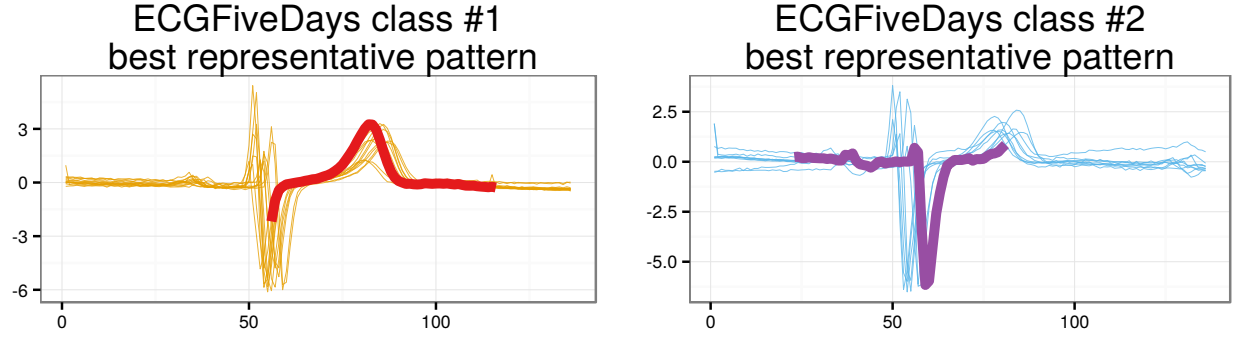
\includegraphics[width=.7\textwidth]{pictures/representativepatterns}
	\caption{``Two classes from the ECGFiveDays dataset and the best representative patterns''~\cite{wang2016rpm}.  Image taken from~\cite{wang2016rpm}.}
	\label{fig:representativepatterns}
\end{figure}

\begin{figure}[H]
	\centering
	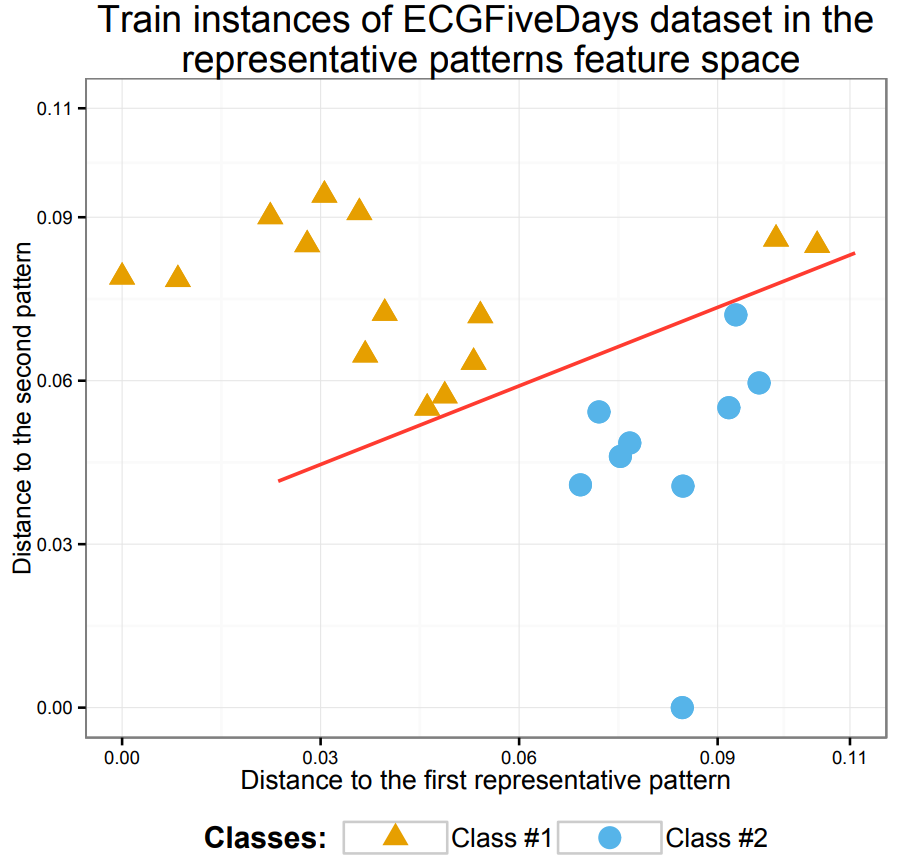
\includegraphics[width=.7\textwidth]{pictures/featurevec}
	\caption{``Transformed data of train data from ECGFiveDays''~\cite{wang2016rpm}.  Image taken from~\cite{wang2016rpm}.}
	\label{fig:featurevec}
\end{figure}


This distance feature vector is then used as the training data to a supervised classifier. TSAT uses Random Forest as the supervised classifier.

In order to set the optimal sliding window size, PAA size, and alphabet length (the SAX Parameter Combinations SPCs) for each class, RPM implements the DIRECT (Dividing Rectangles) parameter optimization algorithm.  The error function is one minus the F1 measure from a five fold cross validation on the validation data.  DIRECT will output the best SPCs so far therefore leaving it to the user to decide the number of iterations of the algorithm to perform.  Leaving the number of iterations to the user is useful as running DIRECT it time intensive as it must perform the motif discovery and training the classifier for each new SPC.  The number of iterations is discussed in more detail in Section~\ref{iterations}.


\subsection{Overview}

The rest of the user manual will go over in detail how to perform motif discovery (Section~\ref{MotifGuide}), anomaly detection (Section~\ref{AnomalyGuide}), and time series classification (Section~\ref{ClassGuide}) using TSAT's GUI.

\section{Motif Discovery}
\label{MotifGuide}

Here the manual will go over the steps on how to format the time series and perform motif discovery in TSAT.  How motif discovery works in TSAT is discussed in Section~\ref{MotifSec} in detail.

\subsection{File format}

In order to perform motif discovery in TSAT the time series must be formatted in a way that TSAT can read.  TSAT requires that the time series be stored in a file where each line in the file contains one entry coresponding to a single time step in the time series.  There must not be any missing lines.  For example a correct file might look like:

\begin{allintypewriter}
	\noindent
	-5.3\\
	2.3\\
	4\\
	42\\
\end{allintypewriter}


\subsection{Guide to Motif Discovery}
%1. Browse for the time series data file and click load data in the data source section
%2. Set the SAX parameters
%	a. manually
%	b. guess (1. click guess 2. click on the time series 3. fill in the fields and click ok 4. wait (make sure to make small enough regions to guess otherwise will take a very long time) 5. )
% Options: Sequitur and RePair
%3. Click Discretize in the Run GI section
%4. Evaluate results by clicking on the grammar rules in the Grammar Rules tab and seeing the subsequences highlighted in the Data Display section and graphed in the Rule Subsequence section

% need to discuss the rule length histogram, cluster rules, and prune rules buttons and what they do as well.


\paragraph{Step 1 (Figure~\ref{fig:step1-browse})} Click ``Browse'' and browse for the time series data file and click ``OK'' when file is selected or ``Cancel'' if you wish to quit browsing.  Then click the ``Load data'' button in the data source section and the time series will be displayed in the Data display section.

\begin{figure}[H]
	\centering
	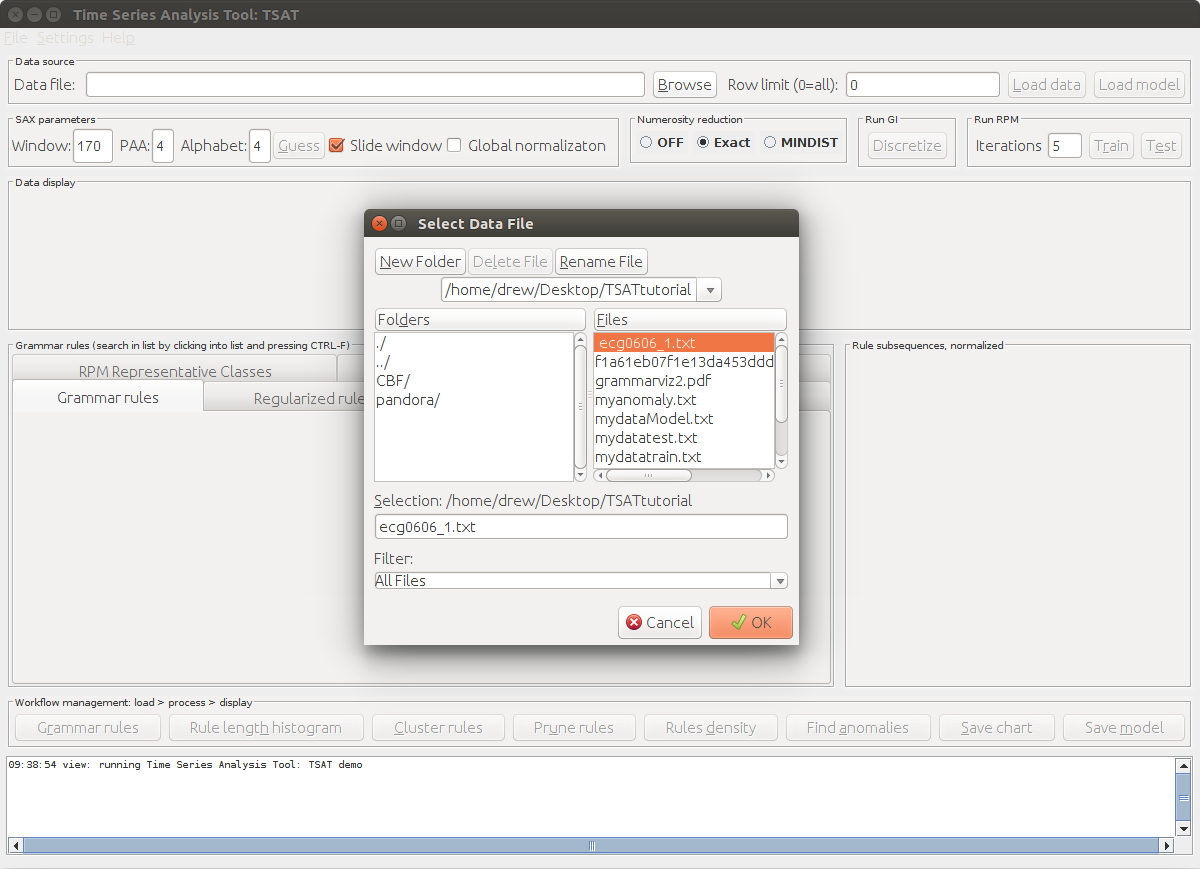
\includegraphics[width=0.7\linewidth]{pictures/motifguide/step1-browse}
	\caption{Click ``Browse'' $\rightarrow$ select file and click ``OK'' $\rightarrow$ click ``Load data''.}
	\label{fig:step1-browse}
\end{figure}


\paragraph{Step 2 (Figure~\ref{fig:step2-loaded})} Set the SAX parameters, ``Window'', ``PAA'', and ``Alphabet'' manually in the ``SAX Parameters'' section and then click ``Discretize'' in the ``Run GI'' section to produce the motifs.  Also, note that you can adjust the numerosity reduction strategy from Exact to either Off or MINDIST and toggling the sliding window and global normalization. How to set the SAX parameters is discussed in Section~\ref{MotifSec}.

\begin{figure}[H]
	\centering
	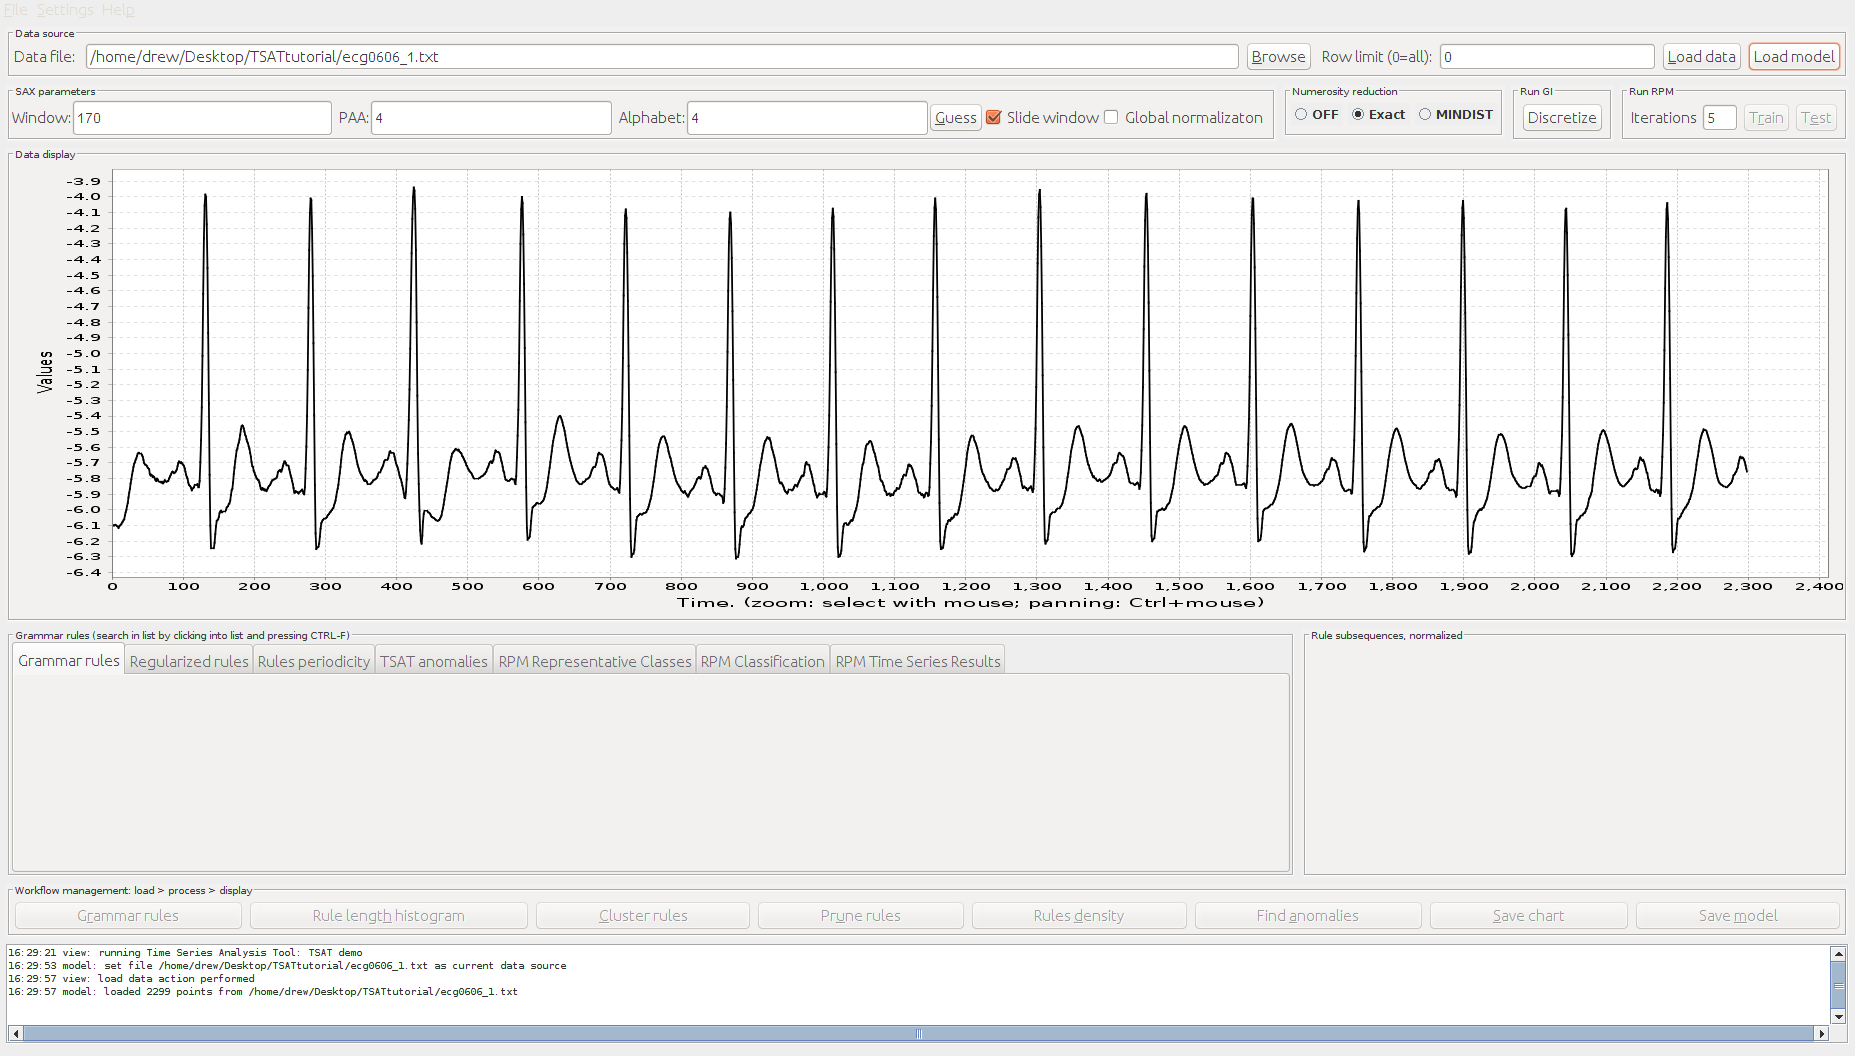
\includegraphics[width=0.7\linewidth]{pictures/motifguide/Step2-loaded}
	\caption{Set SAX Parameters and click ``Discretize''.}
	\label{fig:step2-loaded}
\end{figure}


\paragraph{Step 3 (Figure~\ref{fig:step3-motifs})} Evaluate results by clicking on the grammar rules in the ``Grammar Rules'' tab and seeing the subsequences highlighted in the ``Data Display'' section and graphed in the ``Rule Subsequence'' section.  Each grammar rule row has nine column values: R\#, Level, Frequency in R0, Rule, Expanded Rule, Used, Mean Length, and Min-max length.  These values correspond to:

\begin{description}
	\item[R\#] The rule number where rule number 0 is the root grammar rule.
	\item[Level]  The grammar level or the distance from the root rule.
	\item[Frequency in R0]  The number of times this rule is used in the root rule.
	\item[Rule] The actual grammar rule.
	\item[Expanded Rule]  The grammar rule that has its non-terminal symbols replaced with the terminal symbols.
	\item[Used]  The number of times that rule is used by other rules.
	\item[Mean Length] The average length of the subsequence that this rule spans.
	\item[Min-max Length] The minimum and the maximum length that the rule spans in the time series.
\end{description}

A selected rule or motif found by {\TSAT} is shown in Figure~\ref{fig:step3-motifs}.  Note that multiple rules can be selected by holding the ctrl key and clicking on the rules or holding shift and using the arrow keys to move up and down.

\begin{figure}[H]
	\centering
	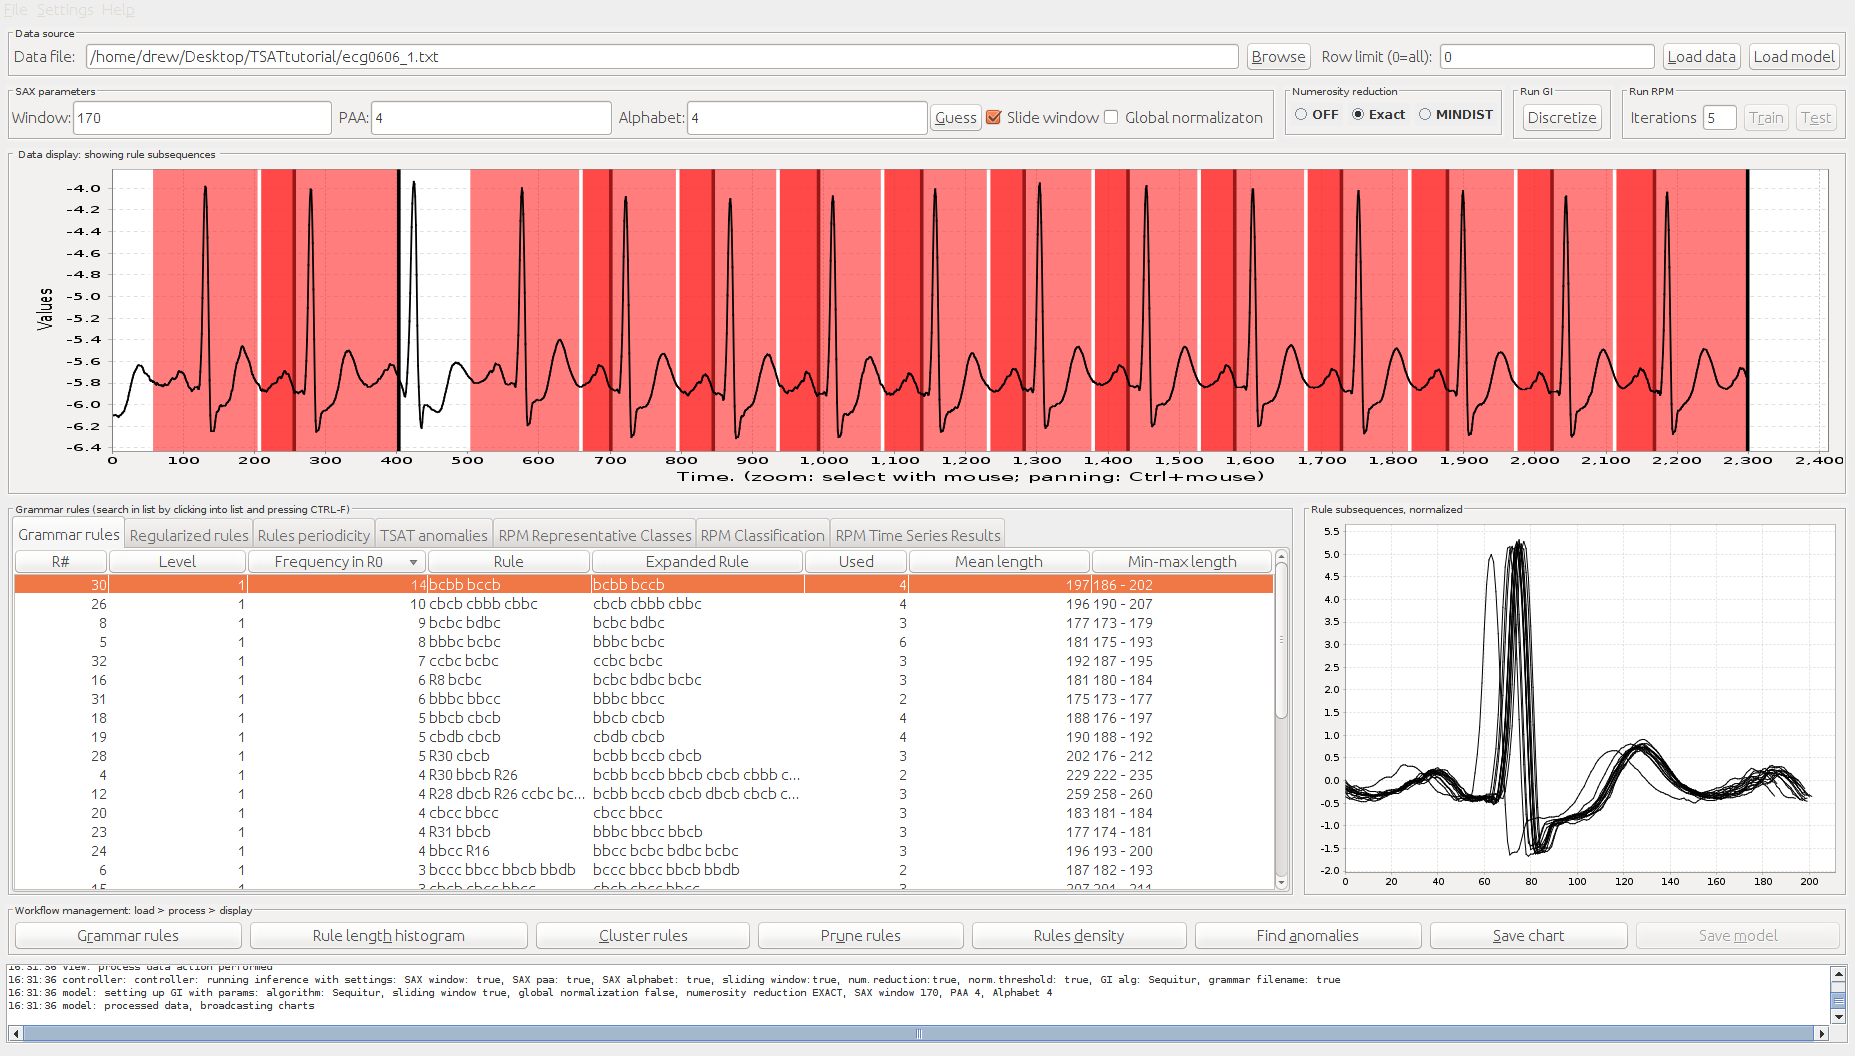
\includegraphics[width=0.7\linewidth]{pictures/motifguide/step3-motifs}
	\caption{List of motifs found by TSAT in the ``Grammar Rules'' tab.  Click on each rule to highlight them in the Data display and graph the subsequence in Rule Subsequence section.  Multiple rules can be selected by holding the ctrl key and clicking on the rules or holding shift and using the arrow keys to move up and down.}
	\label{fig:step3-motifs}
\end{figure}

Additionally, note that by clicking ``Save chart'' in the ``Workflow management'' section {\TSAT} will save a png image of the data display area to a file located in the same directory as the jar file with a file name corresponding to yyyyMMddhhmmssSS.png.

Also, by clicking the ``Rule length histogram'' button in the ``Workflow management'' section {\TSAT} will display a histogram of the rule lengths in Data Display area.



\subsubsection{Guess SAX Parameters}

Rather than manually trying different SAX parameters, TSAT has built in functionality to guess what it perceives as optimal parameters based on user defined range.  This method uses the Re-Pair grammar induction algorithm and the entire process is beyond the scope of this manual but is described in detail in~\cite{paramSelection}.

\paragraph{Step 1 (Figure~\ref{fig:step1-guess})} After loading the dataset from Step 1 in the previous section and instead of setting the SAX parameters manually, click ``Guess.''  This will change the ``Data Display'' to read ``Select the time series interval for guessing.'' Next, Press and hold the left mouse button and drag the mouse across the time series until the desired subsequence of the time series is highlighted and then release the mouse button.  Note that the selected subsequence should be free of anomalies and noise otherwise the guess may produce biases in the results.

\begin{figure}[H]
	\centering
	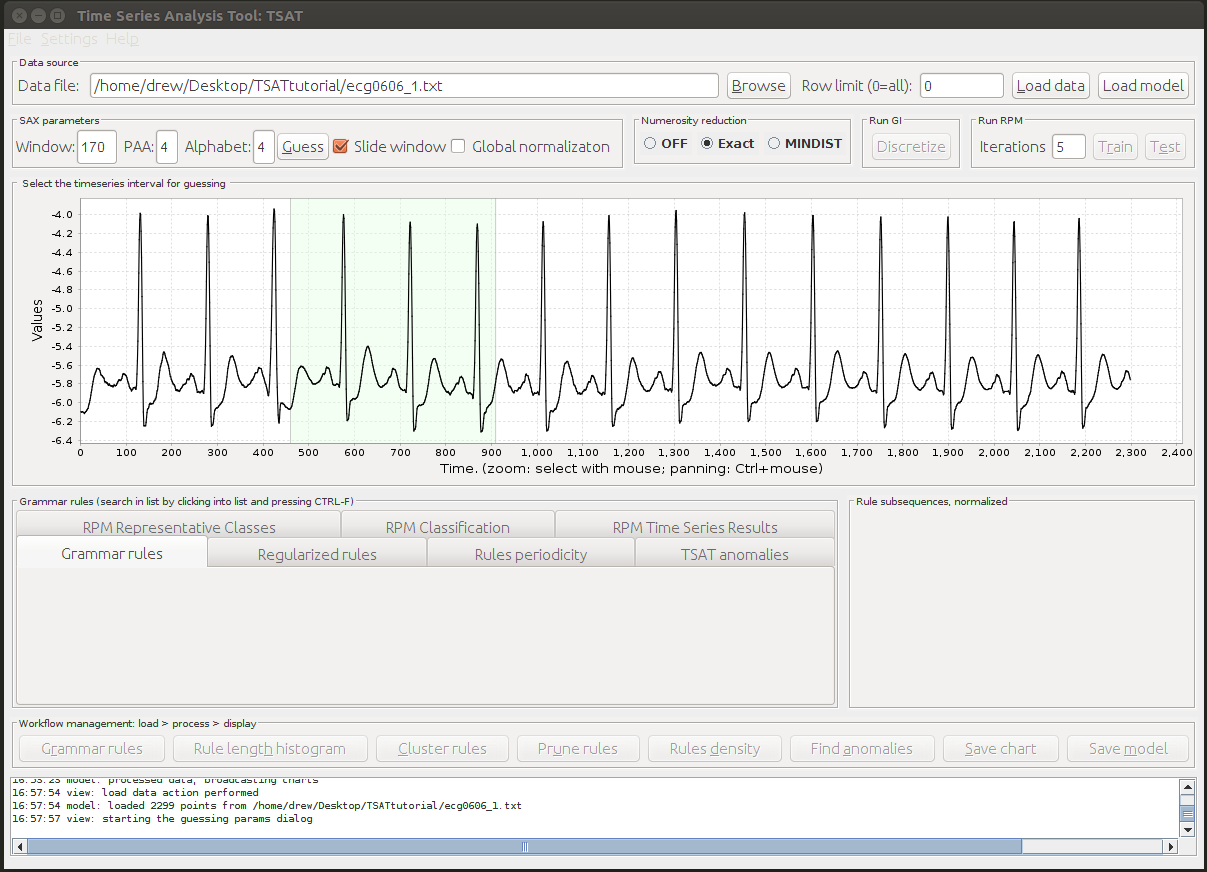
\includegraphics[width=\textwidth]{pictures/motifguide/step1-guess}
	\caption{Click ``Guess'' and then select time series subsequence by clicking and dragging without anomalies or noise.  The green highlighted region is the selected region. }
	\label{fig:step1-guess}
\end{figure}


\paragraph{Step 2 (Figure~\ref{fig:step2-setrange})} After releasing the mouse button a dialog will appear with the title ``Sampler interval and parameter ranges verification.''  Here you may adjust the values as appropriate and then click ``OK'' otherwise if you wish to cancel press ``Cancel.''  

\begin{figure}[H]
	\centering
	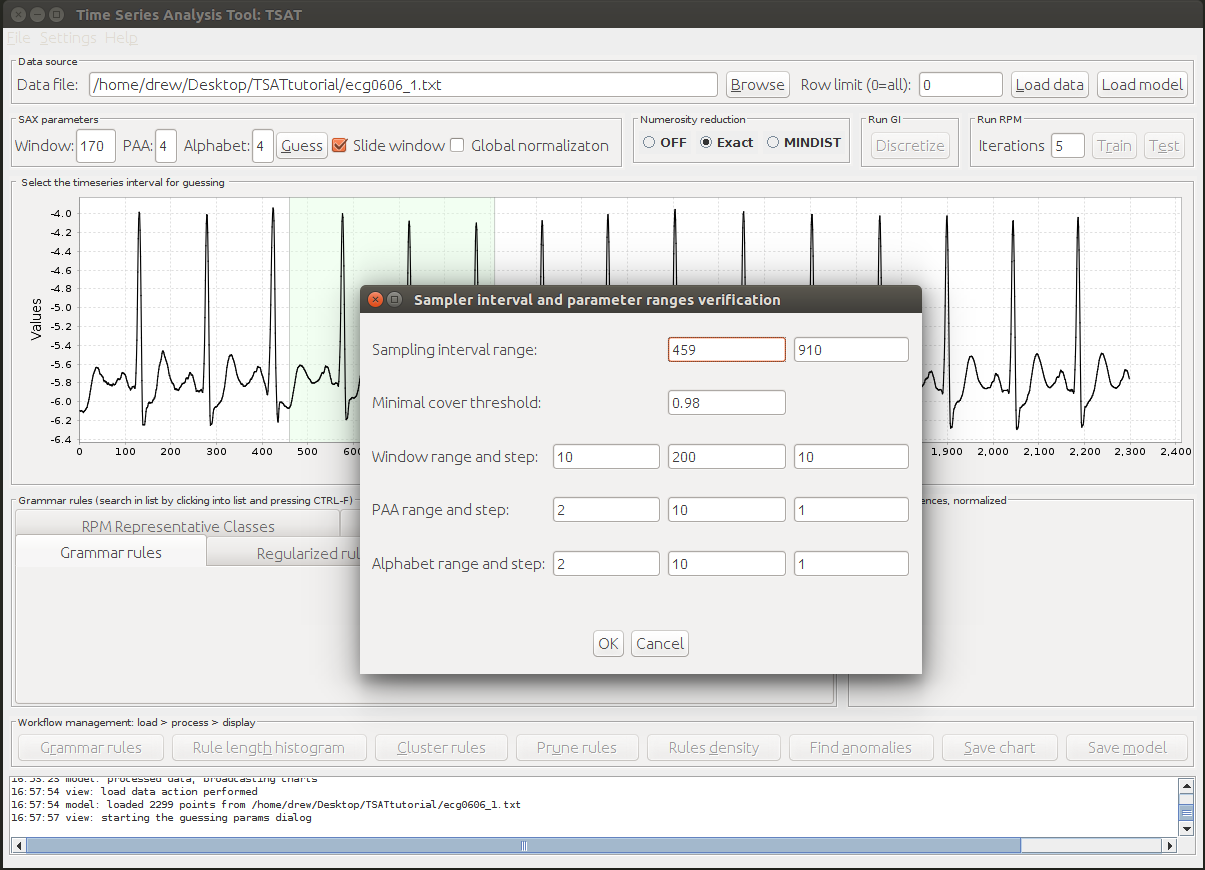
\includegraphics[width=\textwidth]{pictures/motifguide/step2-setrange}
	\caption{Adjust the range values as appropriate to your time series.  Note that the larger the range the longer it will take to search. }
	\label{fig:step2-setrange}
\end{figure}


\paragraph{Step 4 (Figure~\ref{fig:step3-guessresults})} If you  have pressed ``OK'' then the process will beginning and if you wish to stop it press ``stop!'' and TSAT will stop searching for the SAX parameters.  Otherwise after a period of time the values in the ``SAX Parameters'' section will be replaced with the parameters that guessing mechanism found.

\begin{figure}[H]
	\centering
	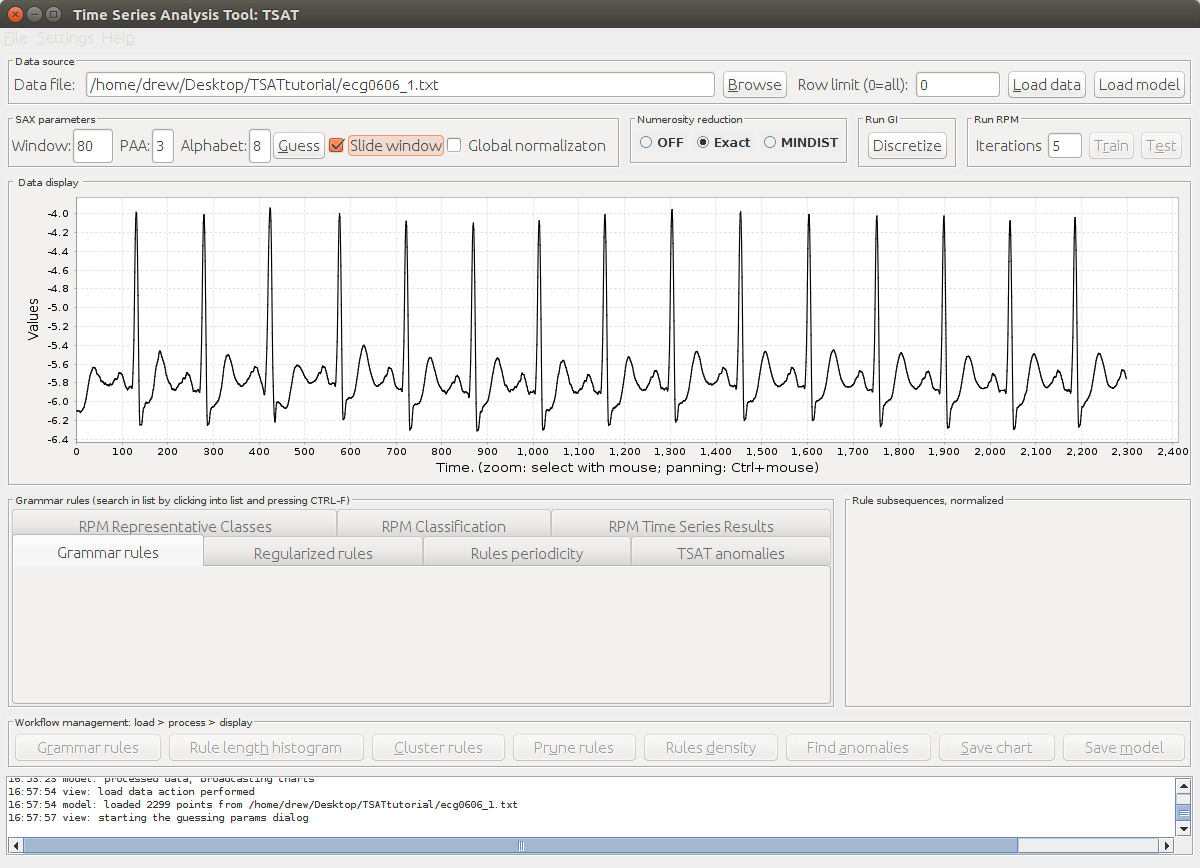
\includegraphics[width=\textwidth]{pictures/motifguide/step3-guessresults}
	\caption{The inferred SAX parameters are filled in the ``SAX parameters'' section.}
	\label{fig:step3-guessresults}
\end{figure}

\subsubsection{Options}

The settings for motif discovery are is accessed by clicking the menu item ``Settings'' and then under that click ``TSAT options'' in order to open the settings.  There are a number of settings including choice of grammar induction, normalization threshold, and location for the output.

\paragraph{Grammar Induction}
The default grammar induction algorithm is Sequitur.  However, RePAIR is also an option. 

Then click on the ``GI Implementation'' tab and the option for RePAIR is presented.  Click on the desired radio button and then click ``save'' to keep your selection or click ``cancel'' to quit.

\paragraph{Normalization Threshold}
The normalization threshold is default value of 0.05 is usually appropriate but is adjustable under the ``Options'' tab.

\paragraph{Output}
Currently the Output tab does not affect the location of output files other than for the Rule density curve filename. 


\subsection{Rule Pruning}

{\TSAT} provides two means for pruning the motifs or the rules: clustering and a greedy pruning algorithm.  Pruning is useful in order to gain better visual insight into the motifs of the time series that are of importance.  This section assumes that the desired time series has been loaded and discretization has been performed following Section~\ref{MotifSec}.

\subsubsection{Clustering Technique}

The clustering method prunes the motifs by classifying the subsequences by length and removing the overlapping in the same length range. This technique is accessed by clicking on the ``Cluster rules'' button in the Workflow management section of the GUI.

Once clicked you are asked for ``threshold for length'' and a ``threshold for overlap.''  The threshold for overlap is not actually currently used.

However the value for the threshold length is used and the subsequences with the length difference within threshold: ``threshouldLength'' will be classified as a class with the function ``classifyMotifs(double)'', i.e. 1-100 and 101-205 will be classified as a class when the threshold is 0.1, because the length difference is 5, which is less than the threshold (0.1 * 100 = 10). If two sub-sequences within one class share a common part which is more than the threshold: ``thresouldCom'', one of them will be removed by the function ``removeOverlappingInSimiliar(double)''. i.e. 1-100 and 21-120.

Once finished the results are presented in the ``Regularized rules'' tab in ``Grammar Rules'' section.

\subsubsection{Greedy Rule Pruning}

The other approach to rule pruning uses a greedy algorithm following a greedy solution of minimum-cardinality set cover problem (an NP-hard problem).  This is an attempt to find the smallest set of rules which cover the most of the input time series in a greedy fashion.  According to~\cite{pruneSite}:
\begin{quote}
	The intuition behind this algorithm is simple -- since our task in hand is to find maximally repeated and minimally-overlapping subsequences (which we consider the most informative), at each iteration, as the best candidate we select the rule which covers the most of the uncovered-so-far time series span thus naturally provides the most information about its structure.
\end{quote}

This functionality is experimental still.  However, it can be used after discretization by clicking ``Prune rules'' in the ``Workflow management'' section of the GUI.  This will update the ``Grammar rules'' tab in the ``Workflow management'' section with the pruned rules.




\subsection{Python Interface}
The python interface for motif discovery is accessed via the buildMotifs function that has the function signature:
\begin{lstlisting}
tsail.buildMotifs(pathToTimeseries, outputFile, window_size=30, word_size=6, alphabet_size=4, strategy="EXACT", threshold=0.01, numworkers=2)
\end{lstlisting}

The parameters are as follows:
\begin{description}
	\item[pathToTimeseries] The path as a string to the location of the time series data
	\item[outputFile] The name of the file that the motifs will be written to.
	\item[window\_size] The SAX parameter for the window size with a default value of 30.
	\item[word\_size] This is the same as the PAA value and indicates the length of the SAX words.  Default word length is 6.
	\item[alphabet\_size] This is the same as Alphabet and indicates the number of characters or symbols that can be chosen.  Default value is 4.
	\item[strategy] This is the numerosity reduction strategy to be used.  The default value of EXACT should be used in most cases.  Other valid values are NONE and MINDIST.
	\item[threshold] SAX normalization threshold meaning that if the input time series' standard deviation is less than this value the z-normalization will not be applied. Default value of 0.01.
	\item[numworkers] This is the number of threads to use when running SAX.  The default value is 2.
\end{description}

For buildMotifs it returns a dictionary where you can index the motifs (or rules generated by Sequitur).

\texttt{<returned\_dict>} is the GrammarRules object that was returned as a result of the call to buildMotifs and has a rules map indexed by the integer rule number starting at \texttt{\bsq{0}}.

\small{\url{https://github.com/jMotif/GI/blob/master/src/main/java/net/seninp/gi/logic/GrammarRules.java}}

\texttt{<returned\_dict>[\bsq{rules}][\bsq{rule\_number}]} will give you a GrammarRuleRecord for a particular \texttt{rule\_number}:

\small{\url{https://github.com/jMotif/GI/blob/master/src/main/java/net/seninp/gi/logic/GrammarRuleRecord.java}}

The list of members accessible in each GrammarRuleRecord follows:

\begin{lstlisting}
/* The rule number in Sequitur grammar. */
private int ruleNumber;


/* The rule string, this may contain non-terminal symbols. */
private String ruleString;

/* The expanded rule string, this contains only terminal symbols. */
private String expandedRuleString;


/* The indexes at which the rule occurs in the discretized time series. */
private ArrayList<Integer> timeSeriesOccurrenceIndexes = new ArrayList<Integer>();


/* This rule intervals on the original time series. */
private ArrayList<RuleInterval> ruleIntervals;


/* The rule use frequency - how many time that rule is used by other rules. */
private int ruleUsageFrequency;

/* The rule level in the hierarchy */
private int ruleLevel;

/* The rule's minimal length. */
private int minLength;

/* The rule's maximal length. */
private int maxLength;

/* The rule mean length - i.e. mean value of all subsequences corresponding to the rule. */
private Integer meanLength;

/* The rule mean period - i.e. the mean length of intra-rule intervals. */
private double period;

/* The rule period error. */
private double periodError;

/* The rule yield - how many terminals it produces in extended form. */
private int ruleYield;
\end{lstlisting}

For example, \texttt{<returned\_dict>[\bsq{rules}][\bsq{1}]} will give you the grammarRuleRecord for rule 1.  The values within the GrammarRuleRecord can then be accessed as you do a python dictionary.

Also, note that ruleIntervals is an array of:

\small{\url{https://github.com/jMotif/GI/blob/32f58578f5a0b184fc836f9d397aa0bfc8e68ee6/src/main/java/net/seninp/gi/logic/RuleInterval.java}}

To access this you just do:\\
\texttt{<returned\_dict>[\bsq{rules}][\bsq{1}][\bsq{ruleIntervals}][<\bsq{rule\_interval\_index}>]}\\
For example,
\texttt{<returned\_dict>[\bsq{rules}][\bsq{1}][\bsq{ruleIntervals}][0]}

Each RuleInterval has the following properties:
\begin{lstlisting}
public int id; // the corresponding rule id
public int startPos; // interval start
public int endPos; // interval stop
public double coverage; // coverage or any other sorting criterion
\end{lstlisting}


\section{Anomaly Detection}
\label{AnomalyGuide}
\subsection{Guide to Anomaly Detection}

This section assumes that you have already performed the steps from Section~\ref{MotifGuide} and have loaded a time series and have produced the motifs.  This section will cover both the approximate and exact forms of anomaly detection using rule density and the Rare Rule Anomaly detection algorithm.


\paragraph{Rules Density} 

After following the steps in Section~\ref{MotifGuide} of loading the dataset and identifying the motifs click the ``Rules Density'' button in the ``Workflow management'' section of the GUI.  Once clicked the results will be displayed in the Data display.  White corresponds to a zero density indicating an anomaly and the darker the color blue the less likely an anomaly exists in that subsequence.  The rule density is displayed in Figure~\ref{fig:ruledensity}.

\begin{figure}[H]
	\centering
	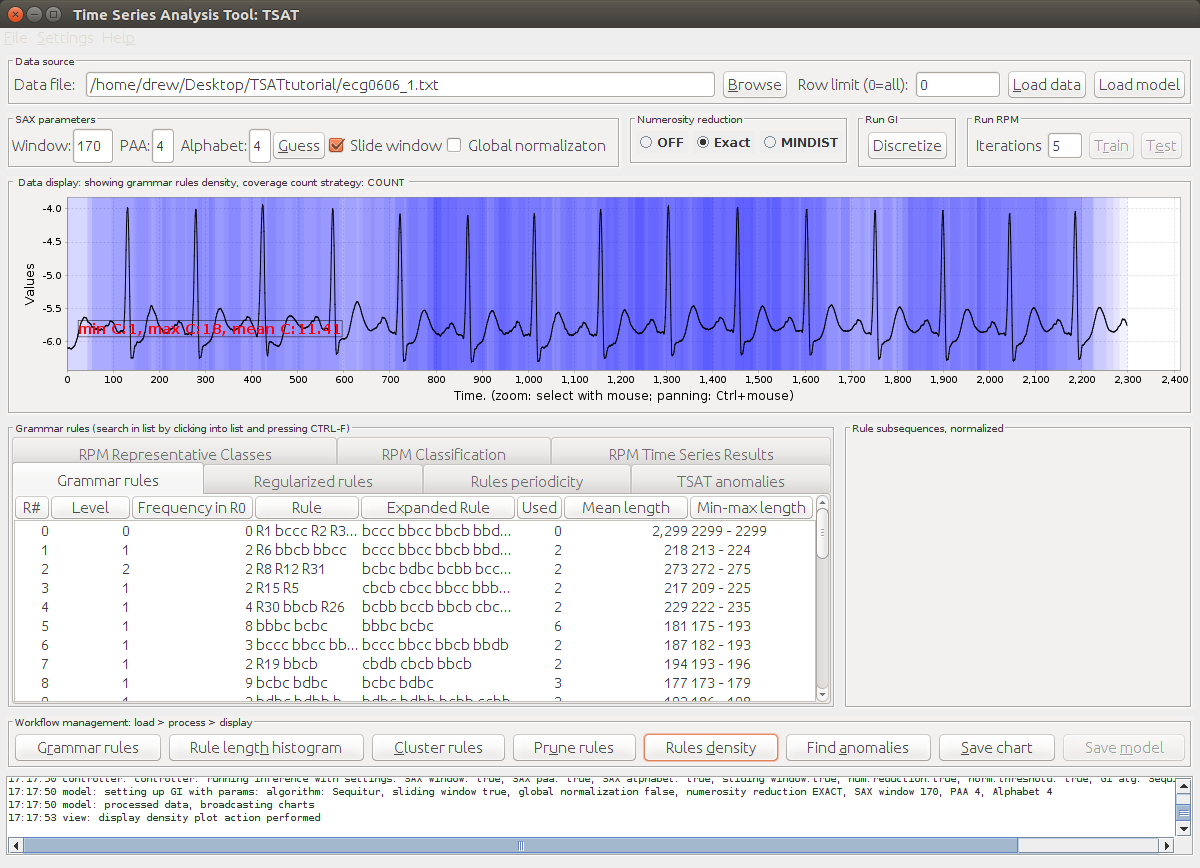
\includegraphics[width=\textwidth]{pictures/motifguide/RuleDensity}
	\caption{Rule density plot in the Data display area.}
	\label{fig:ruledensity}
\end{figure}



By clicking on ``Settings'' and then ``TSAT options'' menu items and a dialog window will appear and you can choose a coverage strategy in the ``Coverage Strategy'' tab (shown in Figure~\ref{fig:coveragestrategy}). Changing the coverage strategy will change how the rule density is calculated.

\begin{figure}[H]
	\centering
	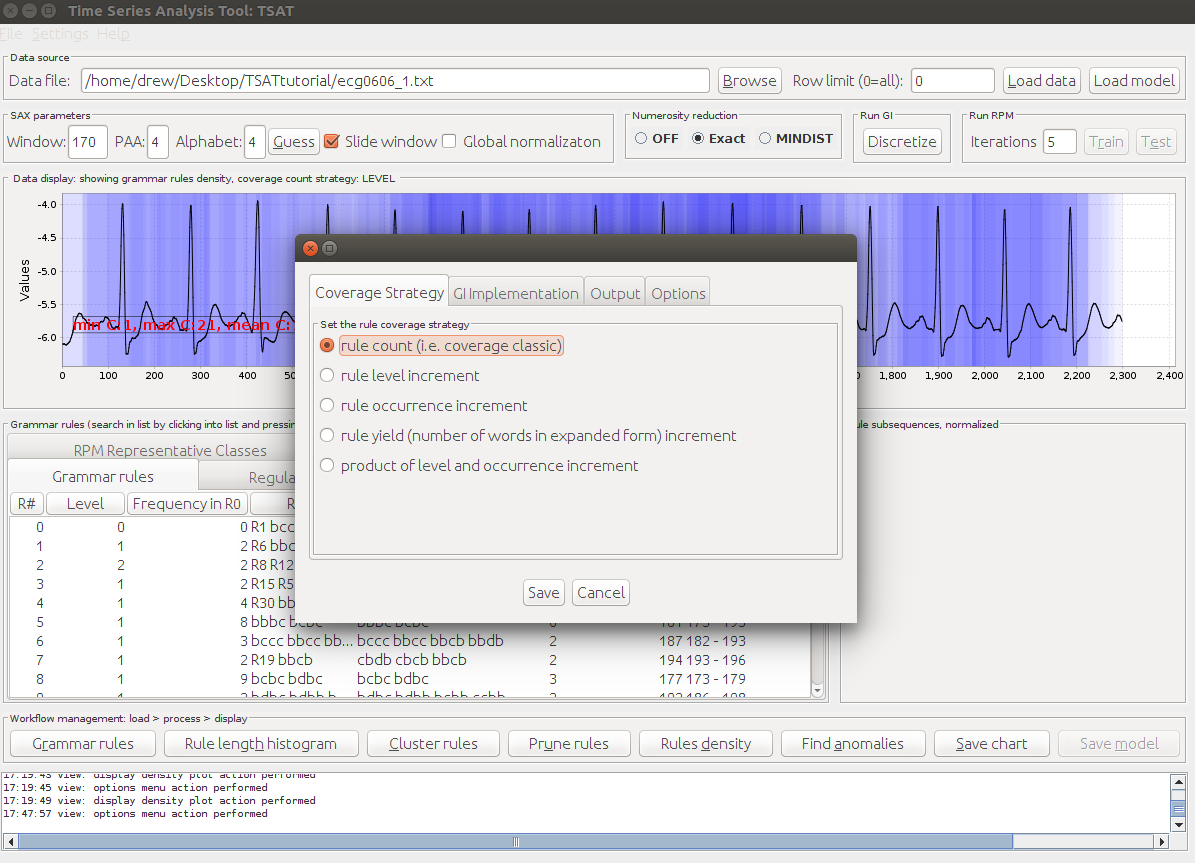
\includegraphics[width=\textwidth]{pictures/motifguide/coveragestrategy}
	\caption{Changing the coverage strategy.}
	\label{fig:coveragestrategy}
\end{figure}

\paragraph{Rare Rule Anomaly Detection}
% Find Anomalies
% Options: Sequitur and RePair

The exact strategy for finding anomalies in {\TSAT} is by using the Rare Rule Anomaly detection algorithm.  This is done by clicking ``Find anomalies'' in the ``Workflow management'' section and then clicking on the ``TSAT anomalies'' tab in the ``Grammar rules'' section.  The top 10 anomalies will be listed in the table in the ``TSAT anomalies'' tab.  Rank, Position, Length, NN Distance, and Grammar Rule are the columns.  Also, when an anomaly is clicked on, the subsequence is highlighted in the Data display and shown in the Rule subsequences section.  Multiple anomalies can be selected by holding Ctrl and then clicking.  The anomaly in the data is shown in Figure~\ref{fig:rraresult}.

\begin{description}
	\item[Rank] The smaller the value the more anomalous the subsequence.
	\item[Position] The start location of the anomaly.
	\item[Length] The length of the subsequence containing the anomaly.
	\item[NN Distance] The distance to the closest subsequence.  The larger this value is the smaller the value Rank is.
	\item[Grammar Rule] The grammar rule that corresponds to the anomaly.  Can return to the Grammar Rules tab and find the rule based on this number.
\end{description}

\begin{figure}[H]
	\centering
	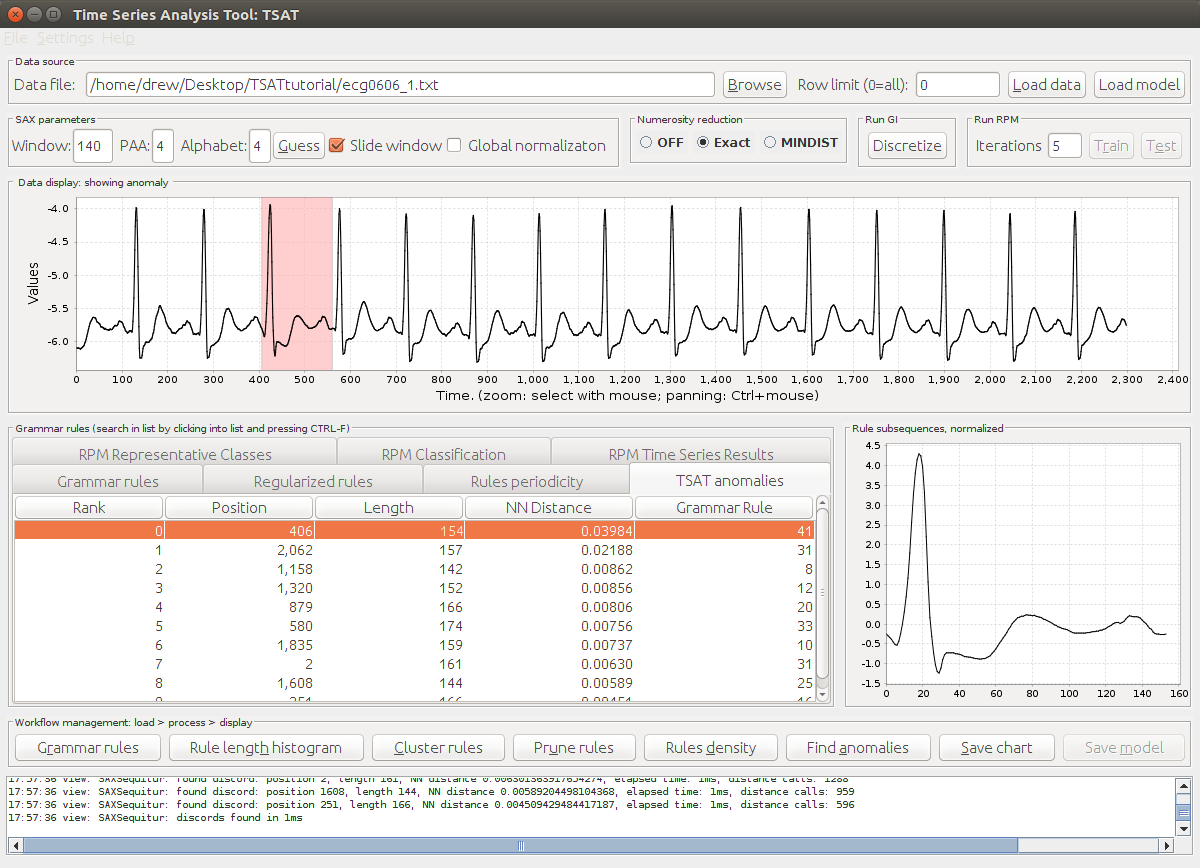
\includegraphics[width=\textwidth]{pictures/motifguide/RRAResult}
	\caption{Rare Rule Anomalies listed in ``TSAT anomalies'' tab.}
	\label{fig:rraresult}
\end{figure}

\subsection{Python Interface}
The function signature for calling anomaly detection using the Rare Rule Anomaly algorithm is:
\begin{lstlisting}
RRA(pathToTimeseries, outputFile, window_size=30, word_size=6, alphabet_size=4, threshold=0.01, discords_num=5)
\end{lstlisting}

With the following parameter definitions:
The parameters are as follows:
\begin{description}
	\item[pathToTimeseries] The path as a string to the location of the time series data
	\item[outputFile] The name of the file that the motifs will be written to.
	\item[window\_size] The SAX parameter for the window size with a default value of 30.
	\item[word\_size] This is the same as the PAA value and indicates the length of the SAX words.  Default word length is 6.
	\item[alphabet\_size] This is the same as Alphabet and indicates the number of characters or symbols that can be chosen.  Default value is 4.
	
	\item[threshold] SAX normalization threshold meaning that if the input time series' standard deviation is less than this value the z-normalization will not be applied. Default value of 0.01.
	\item[discords\_num] This is the number of discords to report.  The default value is 5.
\end{description}
	
Which returns a dictionary holding the discord record.

\texttt{returned\_dict = RRA(...)}

When calling RRA you are returned a dictionary representation of DiscordRecords:

\url{https://github.com/jMotif/SAX/blob/27607baa823df21a10d10e80827ffdd15090cbd9/src/main/java/net/seninp/jmotif/sax/discord/DiscordRecords.java}

Which is a list of DiscordRecord based on:

\url{https://github.com/jMotif/SAX/blob/660e837edf1c8058eac6ef05185c7f83e12f3689/src/main/java/net/seninp/jmotif/sax/discord/DiscordRecord.java}

So, a DiscordRecord can be accessed by doing 
\texttt{<returned\_dict>[\bsq{discords}][0]}

Each DiscordRecord has the following properties:
\begin{lstlisting}
/** The discord id (used when wrapped by RRA). */
private int ruleId;

/** The discord position. */
private int position;

/** The discord length. */
private int length;

/** The NN distance. */
private double nnDistance;

/** The payload - auxiliary variable. */
private String payload;

/** The info string - auxiliary variable. */
private String info;

\end{lstlisting}

For example, length of the DiscordRecord 0 can be accessed as:
\texttt{<returned\_dict>[\bsq{discords}][0][\bsq{length}]}


\section{Time Series Classification using RPM}
\label{ClassGuide}
TSAT implements Representative Pattern Mining or RPM  (see Section~\ref{RPMOverview} for more details) to perform time series classification.  In order to perform time series classification you will need a training and a test dataset containing time series data.

The standard method to train a supervised learning classifier is to take the labeled dataset and split it into two datasets, training and testing data.  One common way to split the data is to have 80\% training and 20\% testing.  

\paragraph{Training Data}
Training data is the primary data and will be used to create a model that can identify similar patterns in new, unlabeled, data. This data must have a label for each time series so that RPM can learn what the labels can look like. This is where the bulk of the data should be set aside for as RPM will need many samples to find representative patterns.

\paragraph{Testing Data}
Testing data is a small subset of the data usually from the same source as the training data, but not found in the training data. This set of data will be used to test the model that RPM made for accuracy or to predict labels for unlabeled test data.

Splitting data into a training and a test set is beyond the scope of this manual and is not done by TSAT. The goal of this section is to first detail the proper file formats for training and testing data in Section~\ref{RPMFile}. Then the proper procedures to train (Section~\ref{RPMTrain}) and test (Section~\ref{RPMTest})are presented step by step along then with a number of other useful features. 

\subsection{File formats}
\label{RPMFile}
File formatting is very important in TSAT and especially when using RPM.  If the file is not in the correct format TSAT will not be able to read the file and may produce unexpected results or error messages.  The data may be formatted by column, row, or following the ARFF file format. Additionally, the labels for the time series may be any string excluding white space and ``?'' as this is reserved for unknown values in test data.

\begin{figure}[h]
	\caption{Examples of RPM Data}
	\label{fig:rpm-data-exs}
	\begin{subfigure}[b]{0.5\textwidth}
		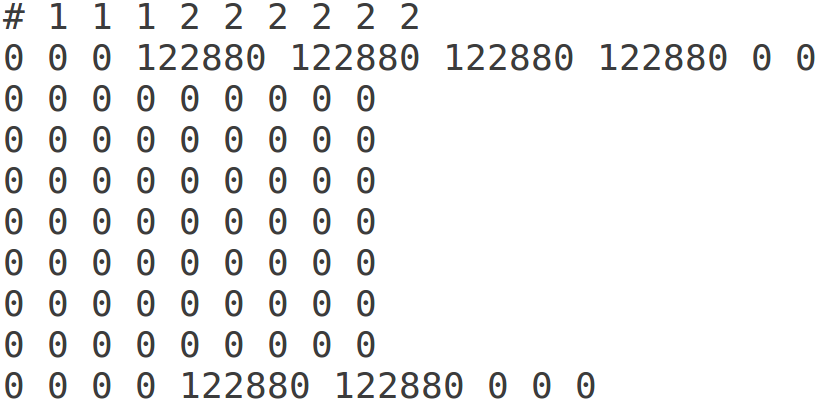
\includegraphics[width=\textwidth]{rpm_data_example_1}
		\caption{Example 1}
		\label{fig:rpm-data-ex-1}
	\end{subfigure}
	~
	\begin{subfigure}[b]{0.5\textwidth}
		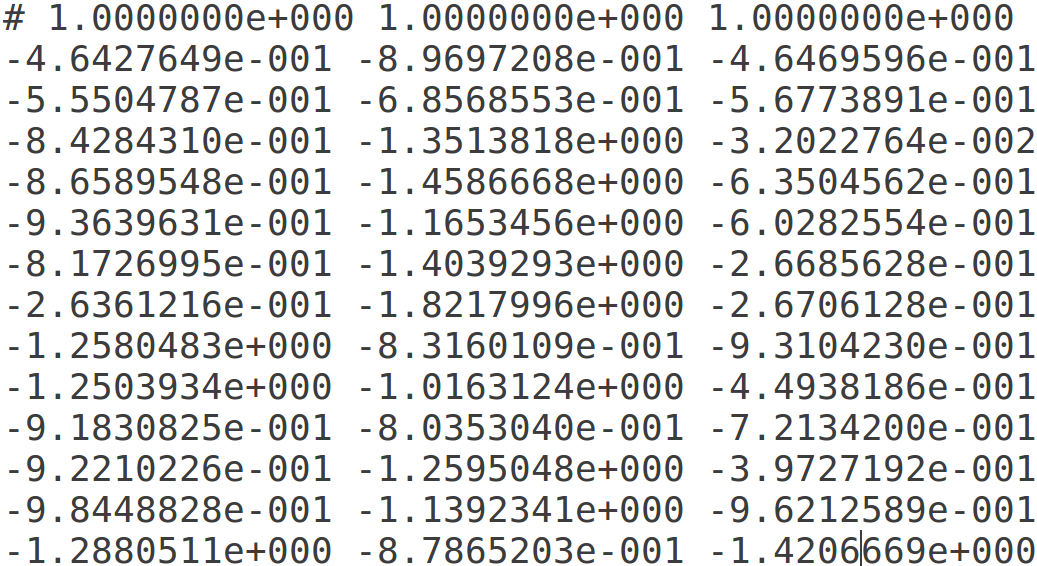
\includegraphics[width=\textwidth]{rpm_data_example_2}
		\caption{Example 2}
		\label{fig:rpm-data-ex-2}
	\end{subfigure}
\end{figure}

\paragraph{Column Formatted Data}
The data files are simple text files that store the time series data with one entry per column, with a space delimiter, with each row representing a time step in the time series data. With RPM compatible data the first row in the file starts with a ``\#'' with rest of the row containing the label for each time series rather then the time series values. If the file is missing this row RPM will not be enabled in TSAT. Examples of column formatted RPM compatible data can be seen in figure~\ref{fig:rpm-data-exs}.  Another thing to keep in mind is that in this format the time series must all be the same length. 

\paragraph{Row Formatted Data}
Another acceptable format is the row format.  This format is especially useful  when the time series are not all the same length as each row or time series may have its own length.  In this format the first line of the file is a ``\#'' followed by a new line.  Starting on the second line, each line starts with the label followed by the corresponding time series (each value separated by a space).  There should be no empty lines.  For example,\\
%\newpage
\begin{allintypewriter}
	\noindent\#\\
	1 -5.3 -23 5 ...\\
	1 23 1 5 3 1 ...\\
	two 23 3 4 200 ...\\
	two 42 3 4 102 ...\\
	...
\end{allintypewriter}
In this example the labels are ``1'' and ``two'' and the time series follow after the labels.

\paragraph{ARFF Formatted data}

A standard format for many public time series datasets is the ARFF file format.  For example, \url{http://timeseriesclassification.com/dataset.php} has a number of time series in ARFF format that can be used in TSAT.  ARFF files are more complicated than both the column and row formats, but is more widely used outside TSAT.  Here is an abbreviated example ARFF file:\\
\begin{samepage}
\begin{allintypewriter}
	\noindent @relation Adiac\\ \\
	@attribute att0 numeric\\
	@attribute att1 numeric\\
	...\\
	@attribute target {1,2,...}\\ \\
	@data\\
	1.3749,1.2894,1.2043,1.1194,1.0347, ... 1\\
	1.7257,1.7001,1.6611,1.6089,1.5319, ... 2\\
	...
\end{allintypewriter}
\end{samepage}
The ARFF file begins with the name of the dataset Adiac by using the ARFF formatting by putting it after the \texttt{@relation} element. After the name of the dataset each timestep is listed as an attribute \texttt{@attribute <timestepName> numeric} where you can choose what to name each timestep. After listing the timesteps as attributes the labels are listed as the target attribute \texttt{@attribute target \{1, 2, ...\}} where these are the labels for the time series. Finally, the time series data is in comma separated value (CSV) format following the \texttt{@data} line.  Each value in a time series is separated by a comma on a single line and the last value on the line is the label for the time series.

\paragraph{Unknown Test Data}
In column, row, or ARFF format when predicting unlabeled test data, the test data must be labeled as ``?'' (note that there must only be test data that is labeled with a ``?'').  For example, a row formatted test dataset might be:

\begin{allintypewriter}
	\noindent\#\\
	? -5.3 -23 5 ...\\
	? 23 1 5 3 1 ...\\
	? 23 3 4 200 ...\\
	...
\end{allintypewriter}

As can be seen the label is ``?'' and the time series follows after the label.  When training there must always be more than one example from each class label and there must be more than one label.

\subsection{Training the Model}
\label{RPMTrain}

Once you have the data in the proper format, training RPM can begin.

\paragraph{Step 1}
First click on the ``Browse'' button under the ``Data Sources'' section of the window, as seen in figure \ref{fig:TSAT-training-step-1}. 

\begin{figure}[h]
	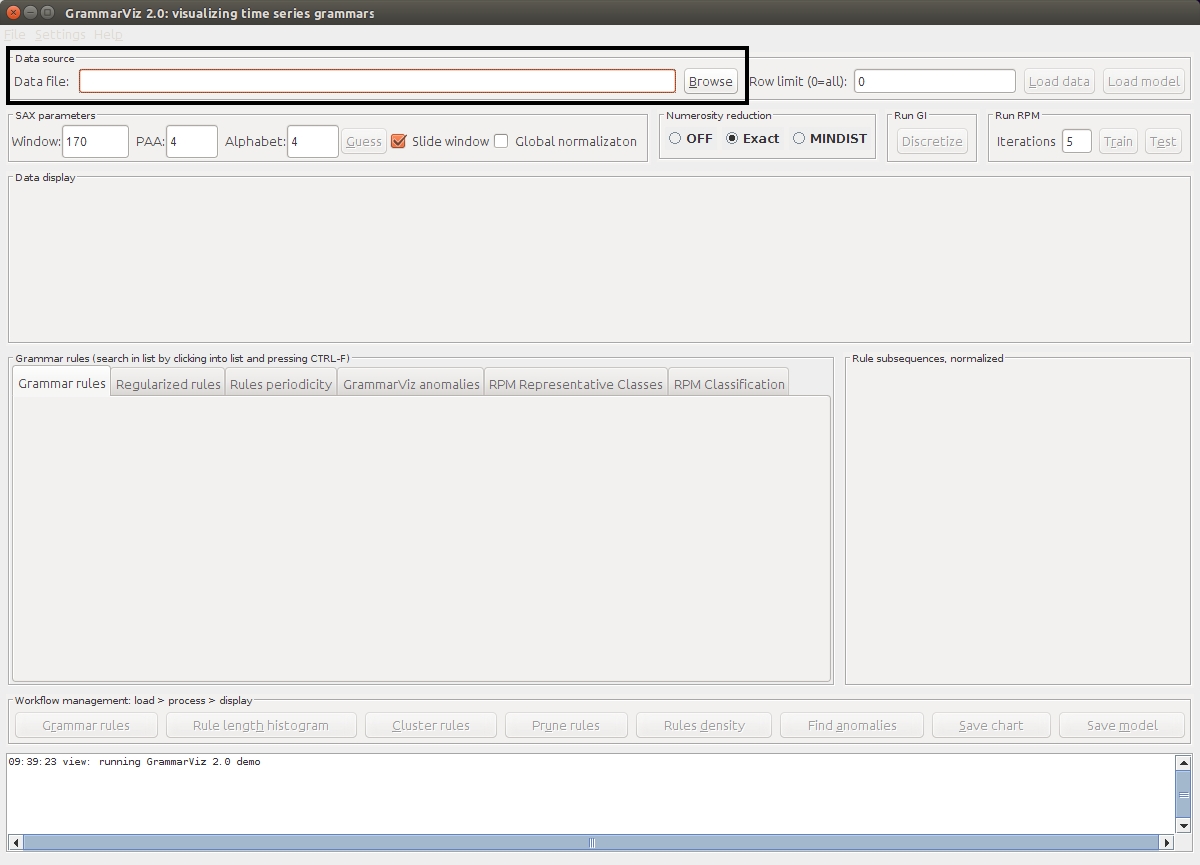
\includegraphics[width=\textwidth]{TSAT-training-step-1}
	\caption{Open TSAT}
	\label{fig:TSAT-training-step-1}
\end{figure}
\newpage
\paragraph{Step 2}
This should bring up the file browser prompt in figure \ref{fig:TSAT-training-step-2}. Using this prompt select the file containing the training set in the RPM compatible format, figure \ref{fig:TSAT-training-step-3}.

\begin{figure}[H]
	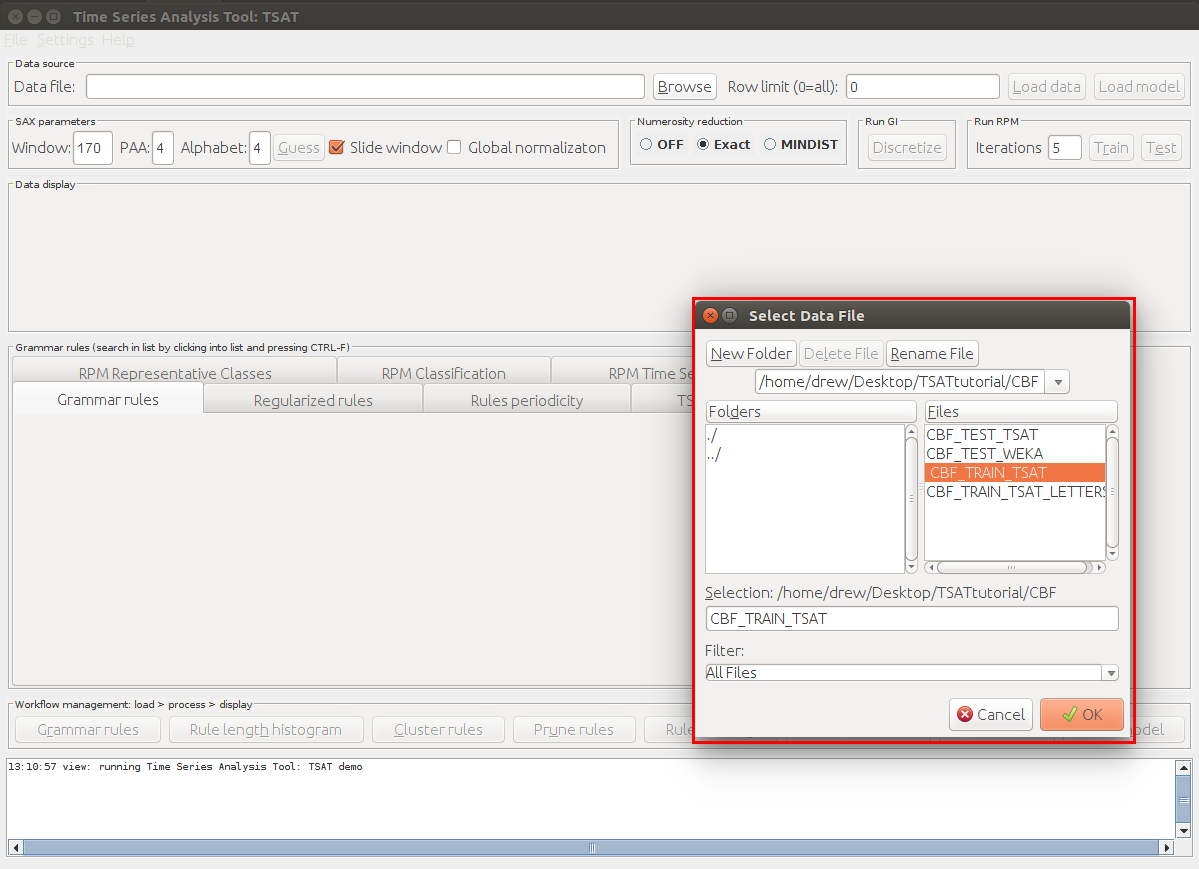
\includegraphics[width=\textwidth]{TSAT-training-step-2}
	\caption{Open the file browser prompt}
	\label{fig:TSAT-training-step-2}
\end{figure}
\begin{figure}[H]
	\center
	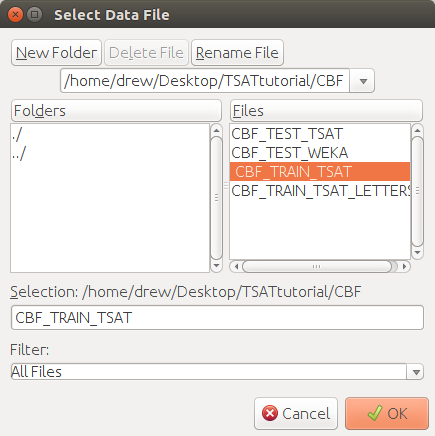
\includegraphics[width=.4\textwidth]{TSAT-training-step-3}
	\caption{Browser prompt}
	\label{fig:TSAT-training-step-3}
\end{figure}

\newpage
\paragraph{Step 3}
After selecting the file press the button labeled ``Load Data'' and  TSAT will load the data and the graphs will be populated, and if the data is found to be RPM compatible data then the ``Train'' button should become available. The text field labeled ``Row Limit'' allows the user to limit the number of rows that are read in from file, for example if the file contains 100 rows the user could limit it to the first 50. 

\begin{figure}[H]
	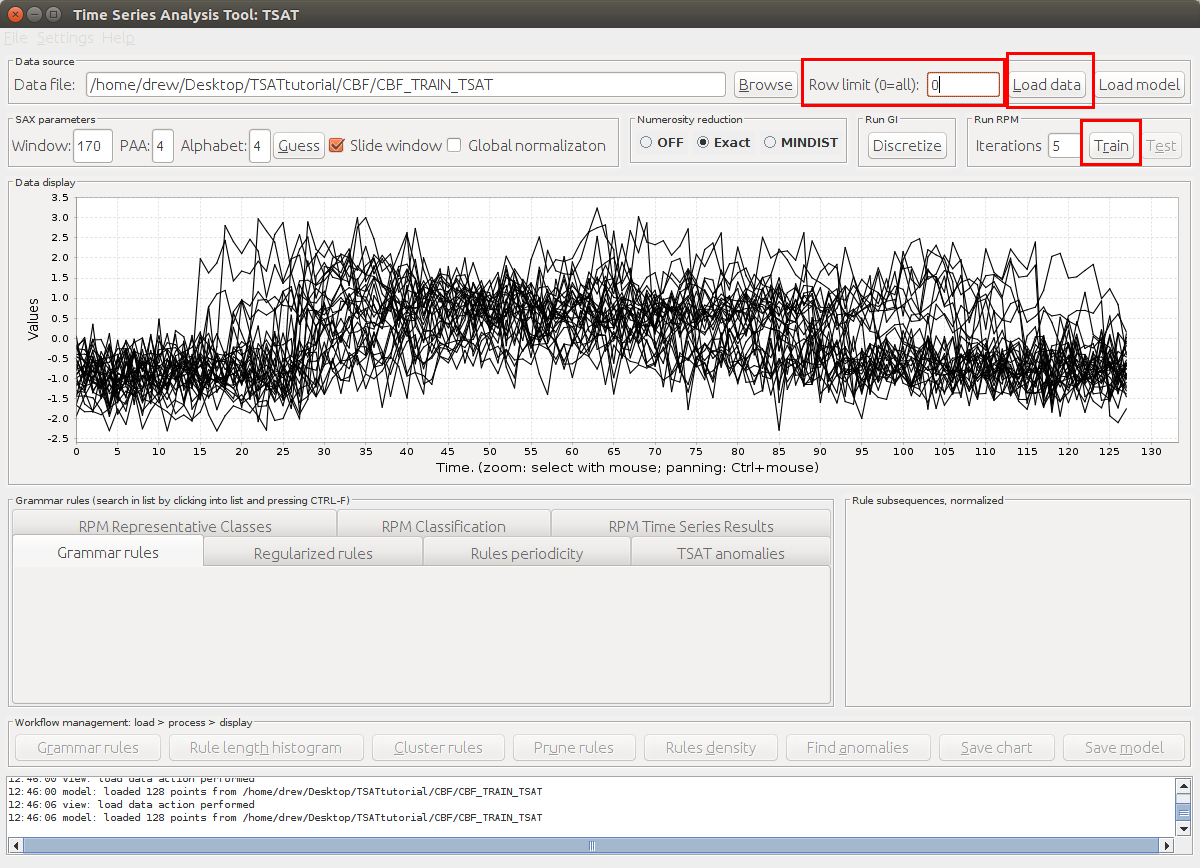
\includegraphics[width=\textwidth]{TSAT-training-step-4}
	\caption{Loaded data}
	\label{fig:TSAT-training-step-4}
\end{figure}

\newpage
Hitting this button will begin the training phase of RPM, this can take some time depending on the data and the number of iterations RPM will run. The text field labeled ``Iterations'' sets the maximum number of iterations RPM will go, this prevents RPM from running for to long trying to refine the model. Once the training is complete the tab ``RPM Representative Classes'' will become populated with patterns RPM thinks be represent the labels given. The fields ``Window'', ``PAA'', and ``Alphabet'' will also be populated with the values RPM believes are the best fit for the data to aid in further analysis. 

\begin{figure}[H]
	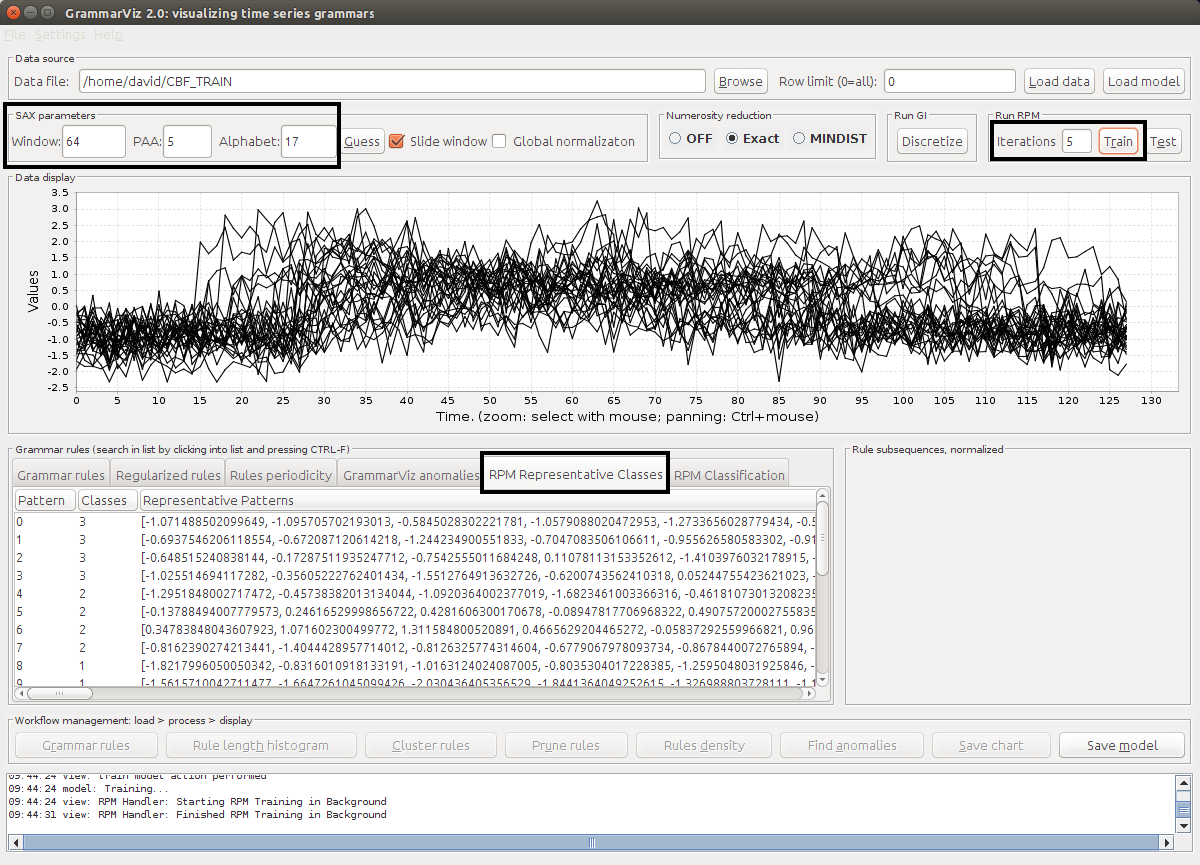
\includegraphics[width=\textwidth]{TSAT-training-step-5}
	\caption{Representative Classes after Training}
	\label{fig:TSAT-training-step-5}
\end{figure}

\newpage
Selecting the patterns will display their graph on the right hand side of the window, multiple patterns can be selected.

\begin{figure}[H]
	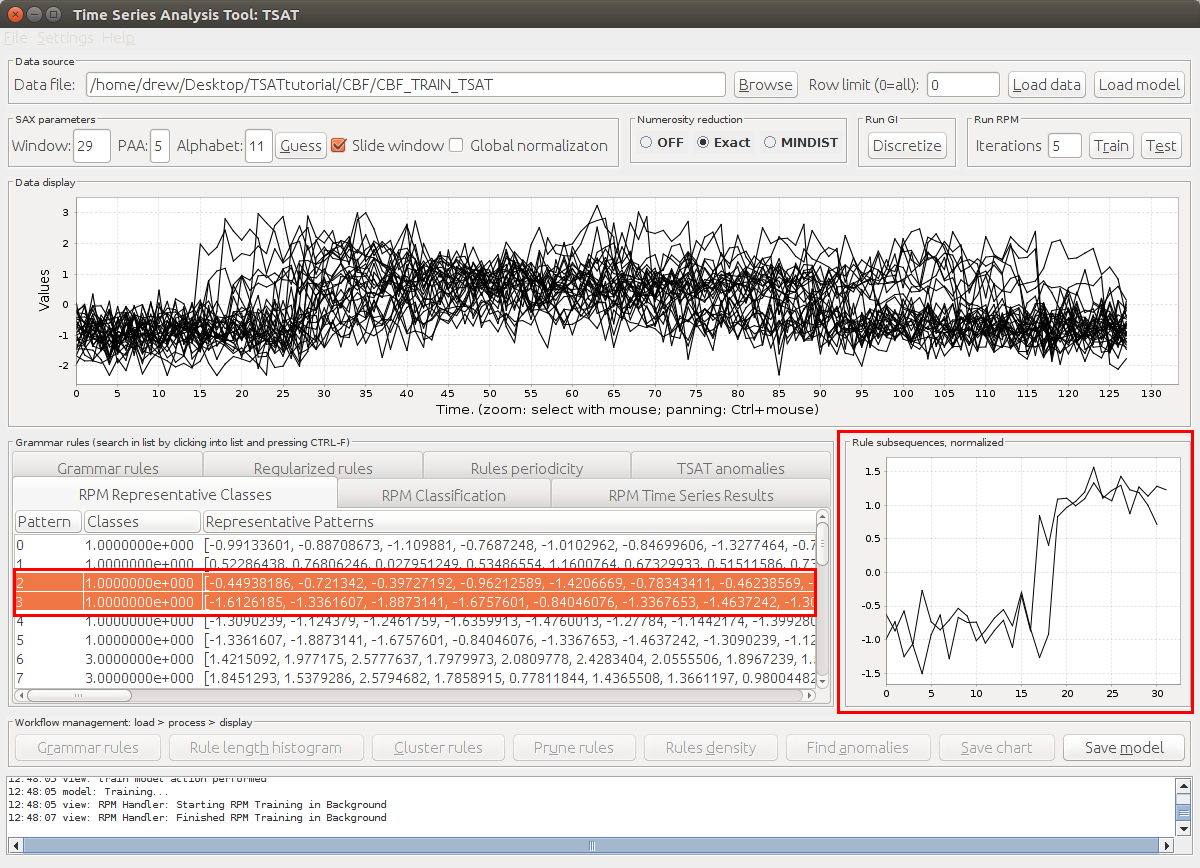
\includegraphics[width=\textwidth]{TSAT-training-step-6}
	\caption{Representative pattern preview}
	\label{fig:TSAT-training-step-6}
\end{figure}


\subsection{Testing}
\label{RPMTest}
Once the model has be trained it should be tested for accuracy, this will use a smaller dataset in the RPM compatible format to measure how well the model does. 

\paragraph{Step 1}
Click the ``Test'' button and a file browser prompt will appear, depending on how large the dataset is this may take a moment. 

\begin{figure}[H]
	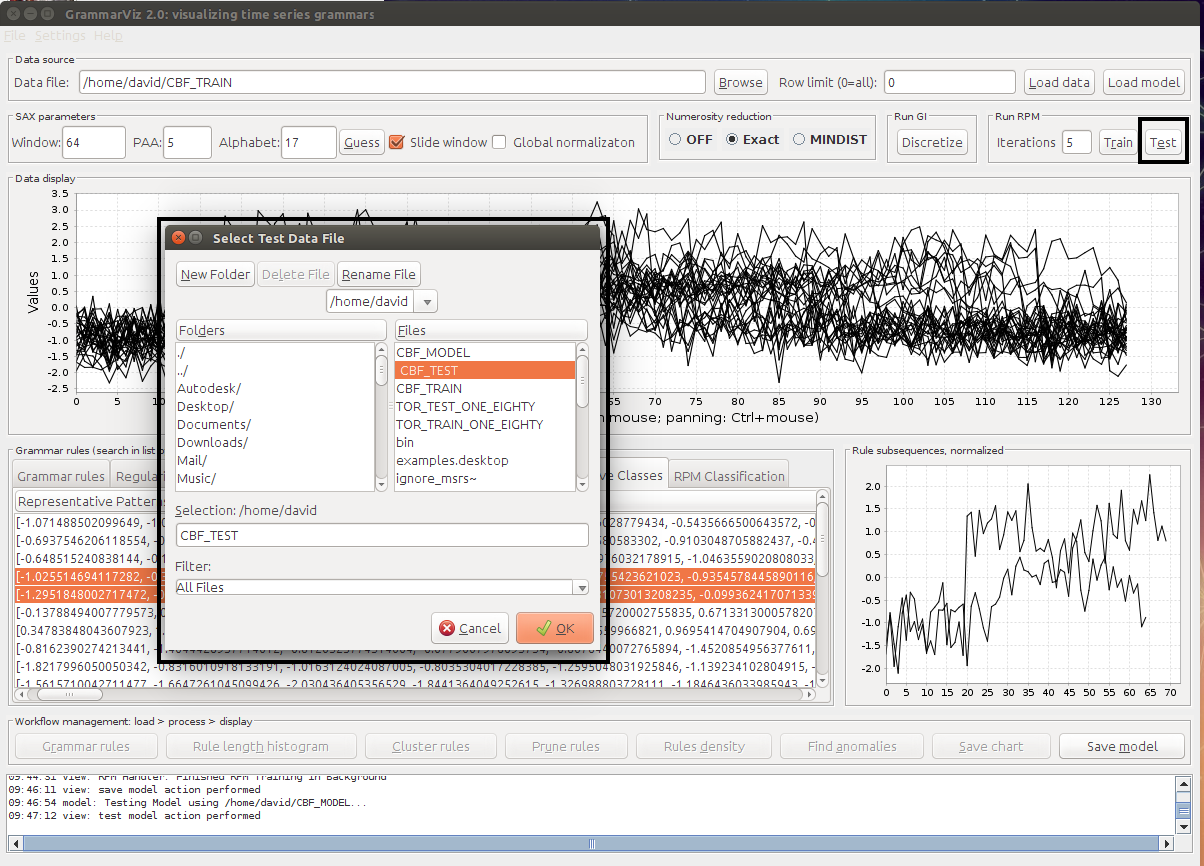
\includegraphics[width=\textwidth]{TSAT-testing-step-1}
	\caption{Testing the RPM model}
	\label{fig:TSAT-testing-step-1}
\end{figure}

\newpage
Once the testing is complete the tab labeled ``RPM Classification'' will be populated. This provides statistics on the effectiveness of the model by reporting the number of samples that were incorrectly labeled by the model.

\begin{figure}[H]
	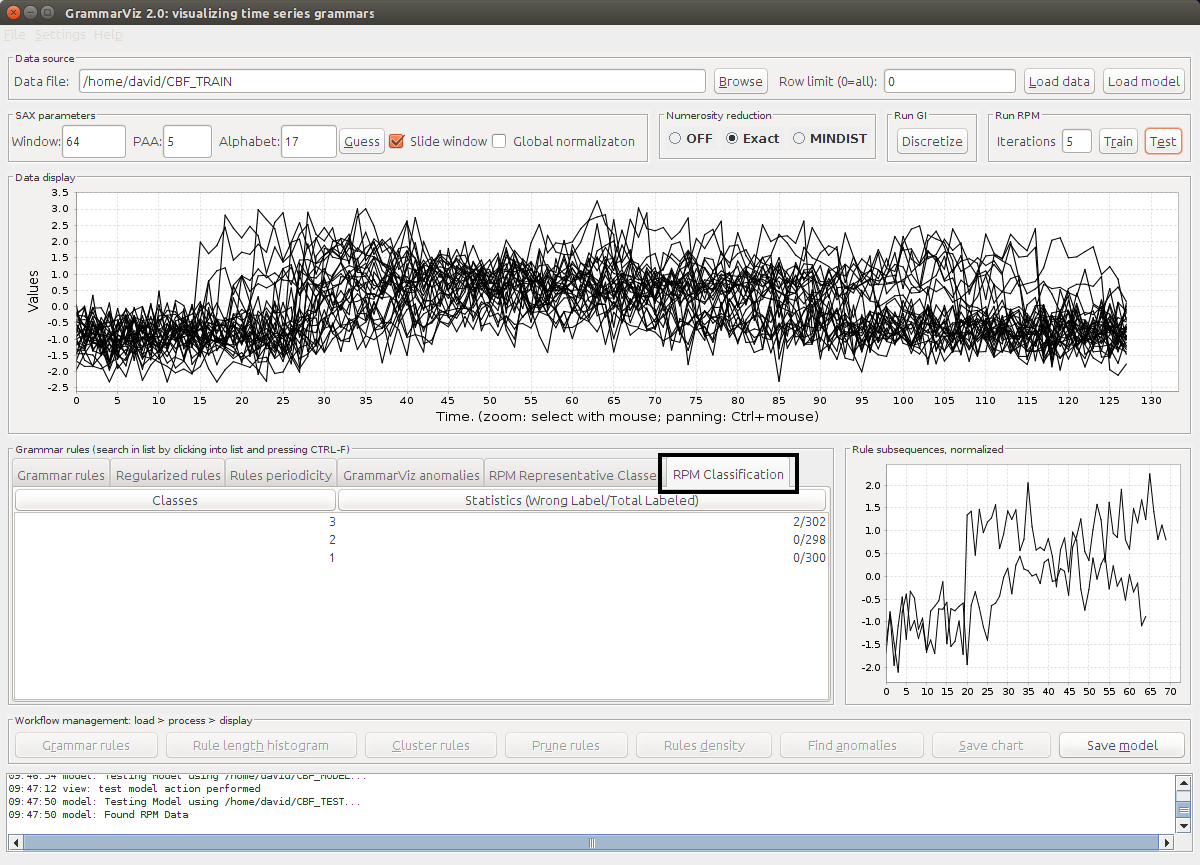
\includegraphics[width=\textwidth]{TSAT-testing-step-2}
	\caption{The results from the testing}
	\label{fig:TSAT-testing-step-2}
\end{figure}

Additionally, under the ``RPM Time Series Results'' tab shows the list of time series that were predicted incorrectly along with the the actual class the time series belongs, the predicted class, time series ID, and the time series.  Shown in Figure~\ref{fig:TSAT-testing-step-3}.

\begin{figure}[H]
	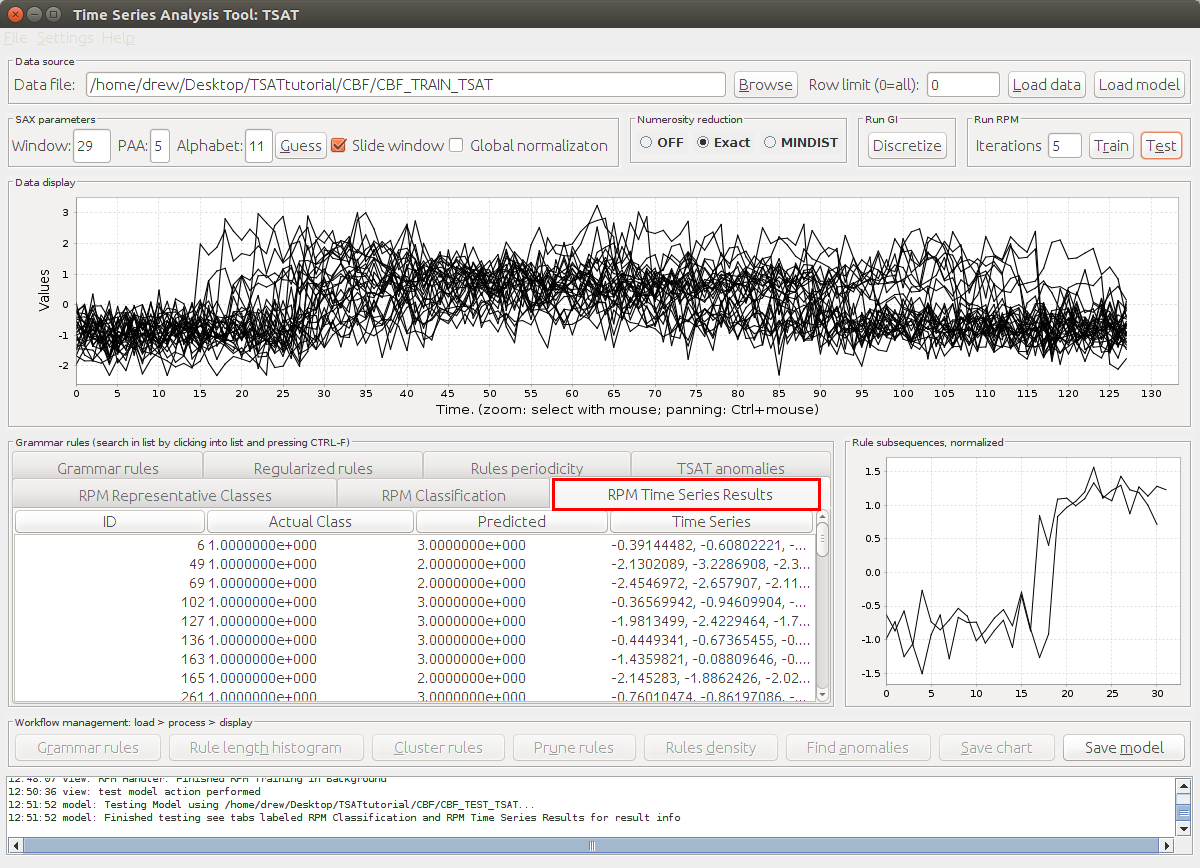
\includegraphics[width=\textwidth]{TSAT-testing-step-3}
	\caption{The results from the testing}
	\label{fig:TSAT-testing-step-3}
\end{figure}

\subsection{Testing Unlabeled Data}
Using the same method for loading the test data when the data is labeled we can see the results for unlabeled data.  Here the test data labels are all question marks so the results will consist of the probability that the test example is in each of the different training classes and the predicted label.  For example, in figure \ref{fig:TSAT-Results-Unknown-Test} the solid box has the label probability for each class and dashed box has the predicted class label.
\begin{figure}[H]
	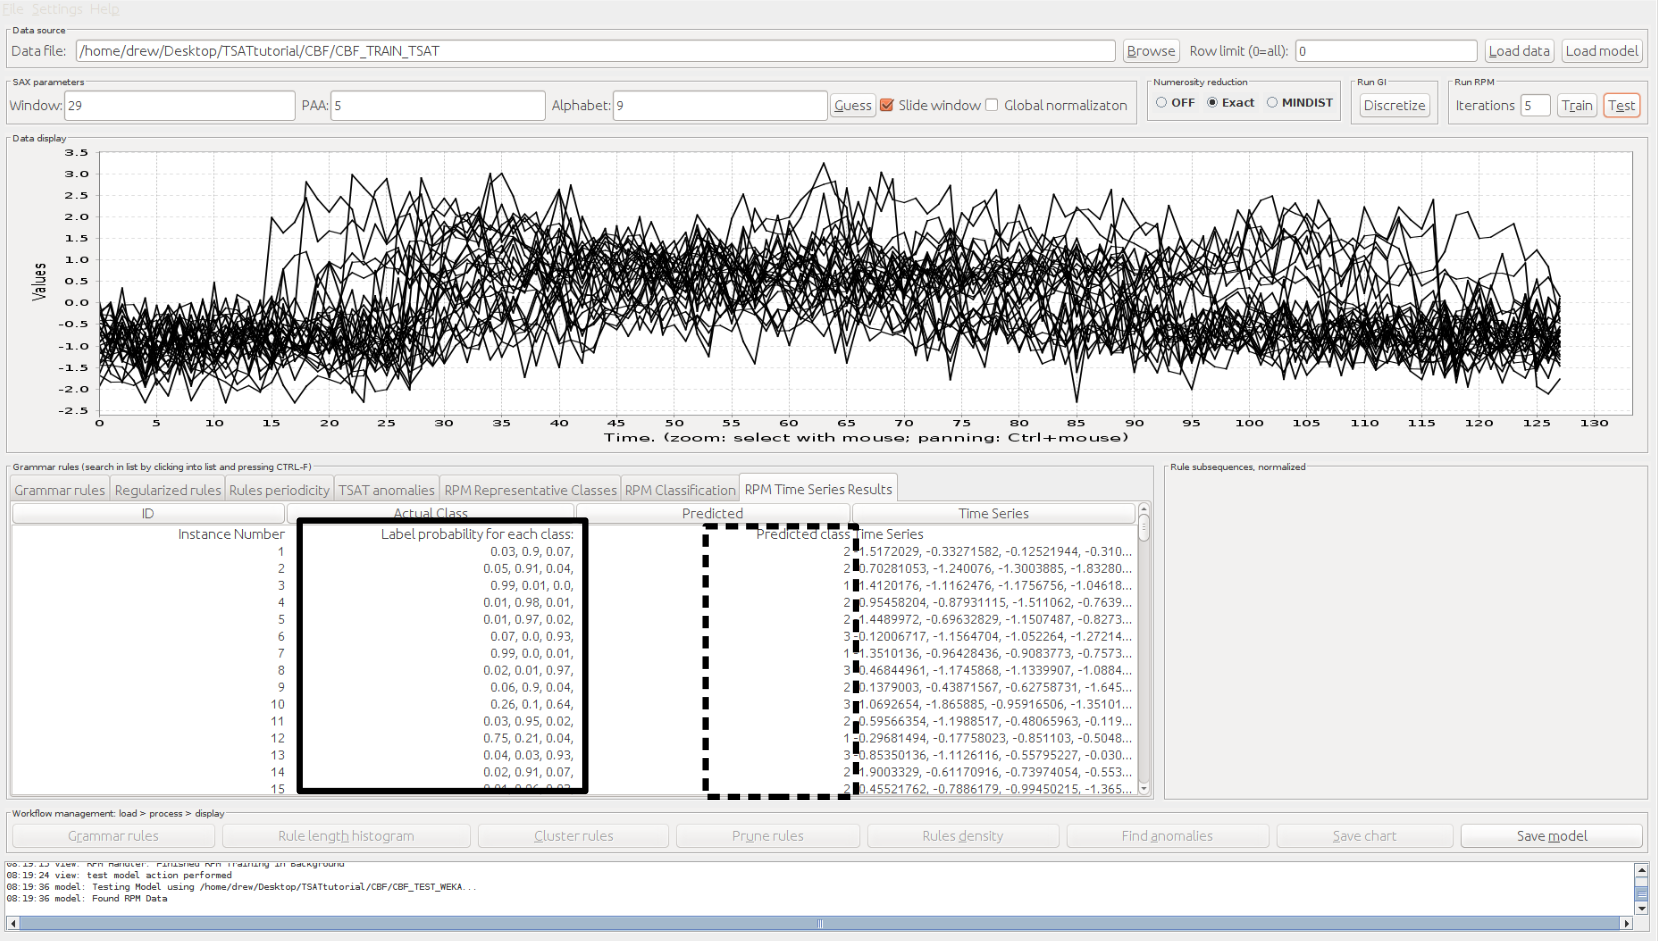
\includegraphics[width=\textwidth]{RPMTimeSeriesResultsUnknown}
	\caption{Solid box highlights the probability that the time series was in each of the different class labels and the dashed box highlights the predicted label.}
	\label{fig:TSAT-Results-Unknown-Test}
\end{figure}

\subsection{Saving a Trained RPM Model}
\label{RPMSaving}
Creating a model can take some time and there for being able to save the model for later uses is a useful feature. Saving the RPM model will generate a file that can be loaded in later for further testing. One thing to note is that the saved model does not contain the training data however the training data is still needed when doing testing there for a copy of the training data must be retained.

\paragraph{Step 1}
Once a model has been trained up clicking the save model button, as in figure \ref{fig:TSAT-save-model-step-1}, a file browser prompt will appear.

\begin{figure}[H]
	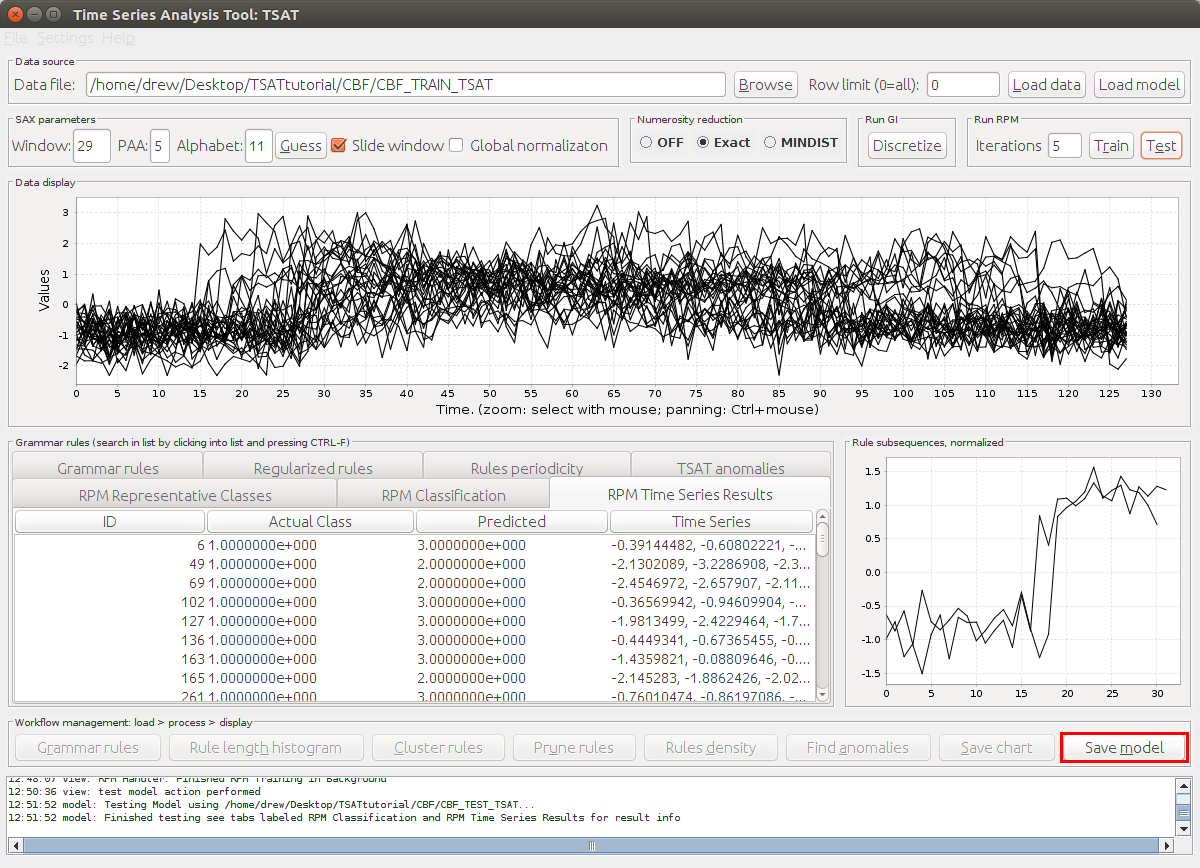
\includegraphics[width=\textwidth]{TSAT-save-model-step-1}
	\caption{Saving the RPM model}
	\label{fig:TSAT-save-model-step-1}
\end{figure}

\newpage
\paragraph{Step 2}
With the file browser prompt select a location to save the model and give it a name, then click the ``OK'' button to save the model.

\begin{figure}[H]
	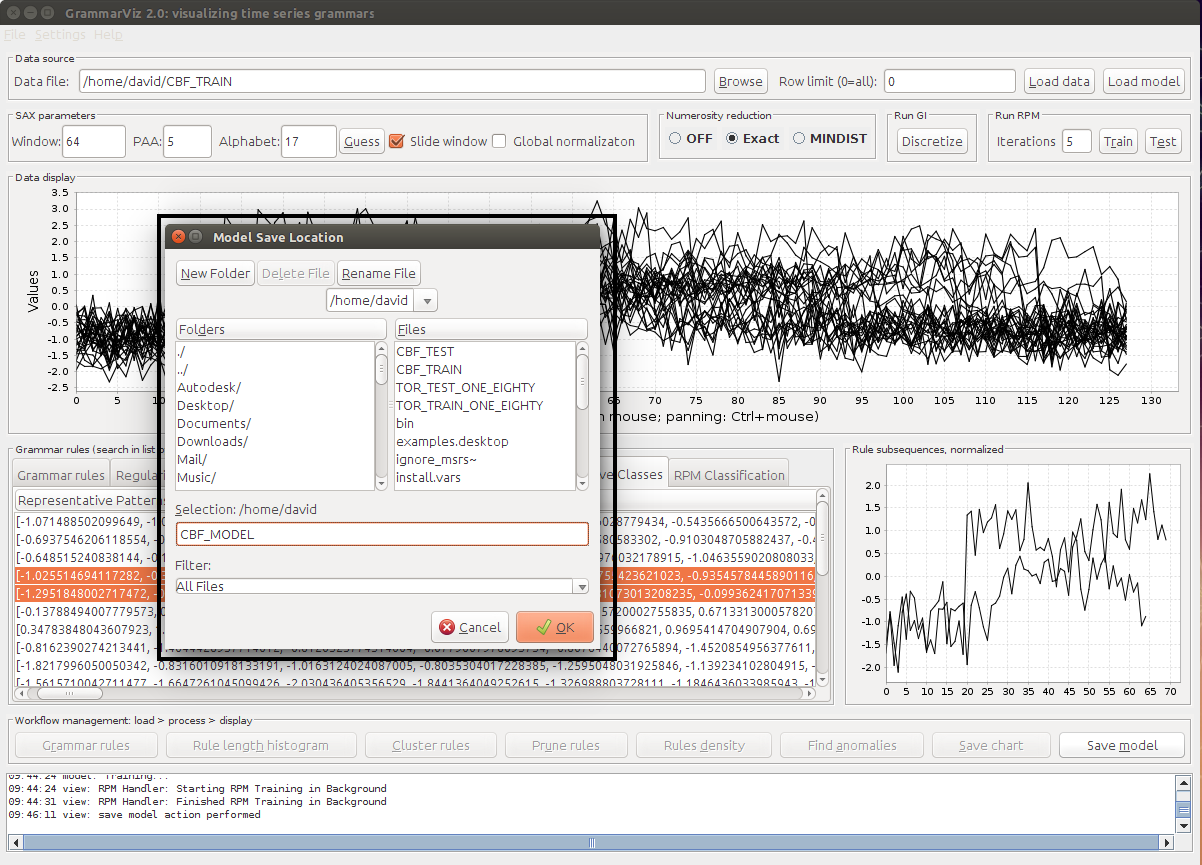
\includegraphics[width=\textwidth]{TSAT-save-model-step-2}
	\caption{Saving the RPM model to file}
	\label{fig:TSAT-save-model-step-2}
\end{figure}

\newpage
\subsection{Loading an RPM Model}
\label{RPMLoading}
When a model has already been saved, simply loading the will allow for further testing. When loading a model the software will look for the original training data from where it was when it was originally trained. If the data is not there then the software will ask for the location of the data.

\paragraph{Step 1}
First click on the ``Browse'' button under the ``Data Sources'' section of the window, as seen in figure \ref{fig:TSAT-load-model-step-1}. 

\begin{figure}[h]
	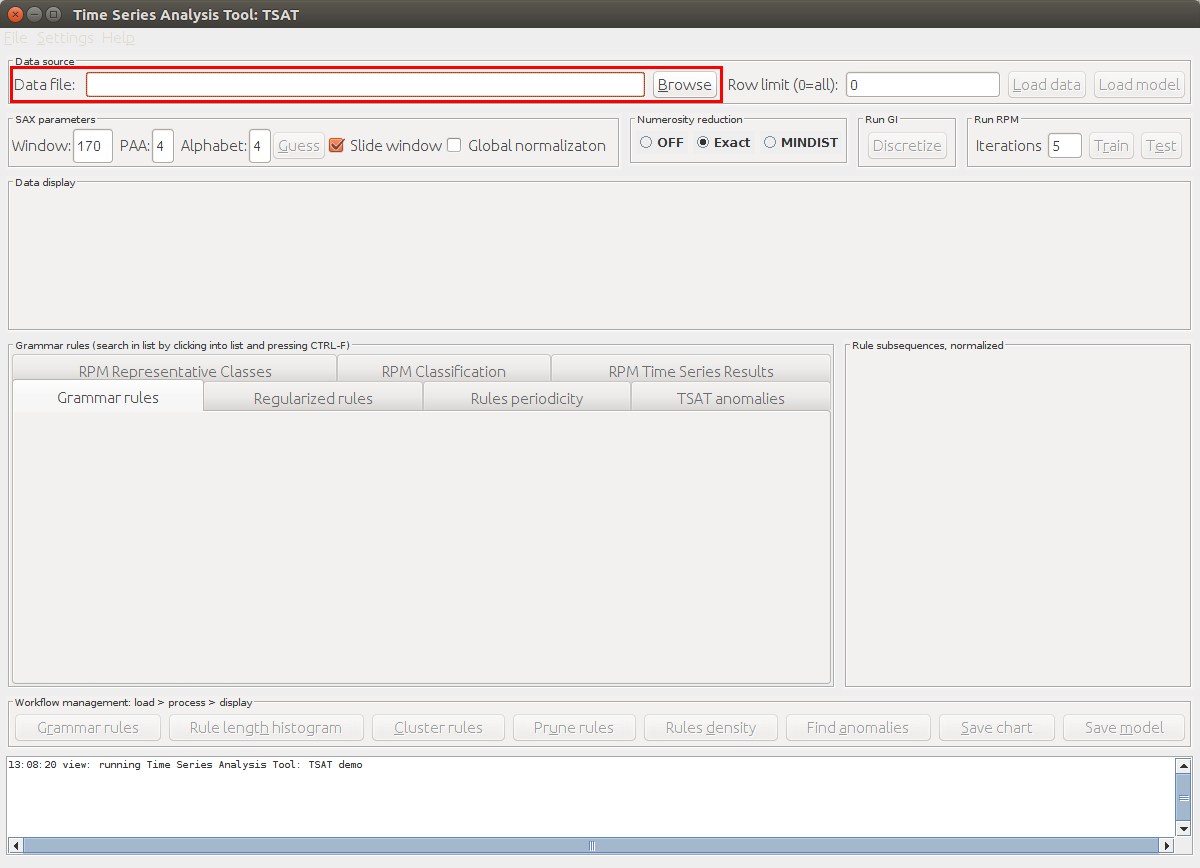
\includegraphics[width=\textwidth]{TSAT-load-model-step-1}
	\caption{Loading a model}
	\label{fig:TSAT-load-model-step-1}
\end{figure}

\newpage
\paragraph{Step 2}
This should being up the file browser prompt in figure \ref{fig:TSAT-load-model-step-2}. Using this prompt select the previously saved model.

\begin{figure}[H]
	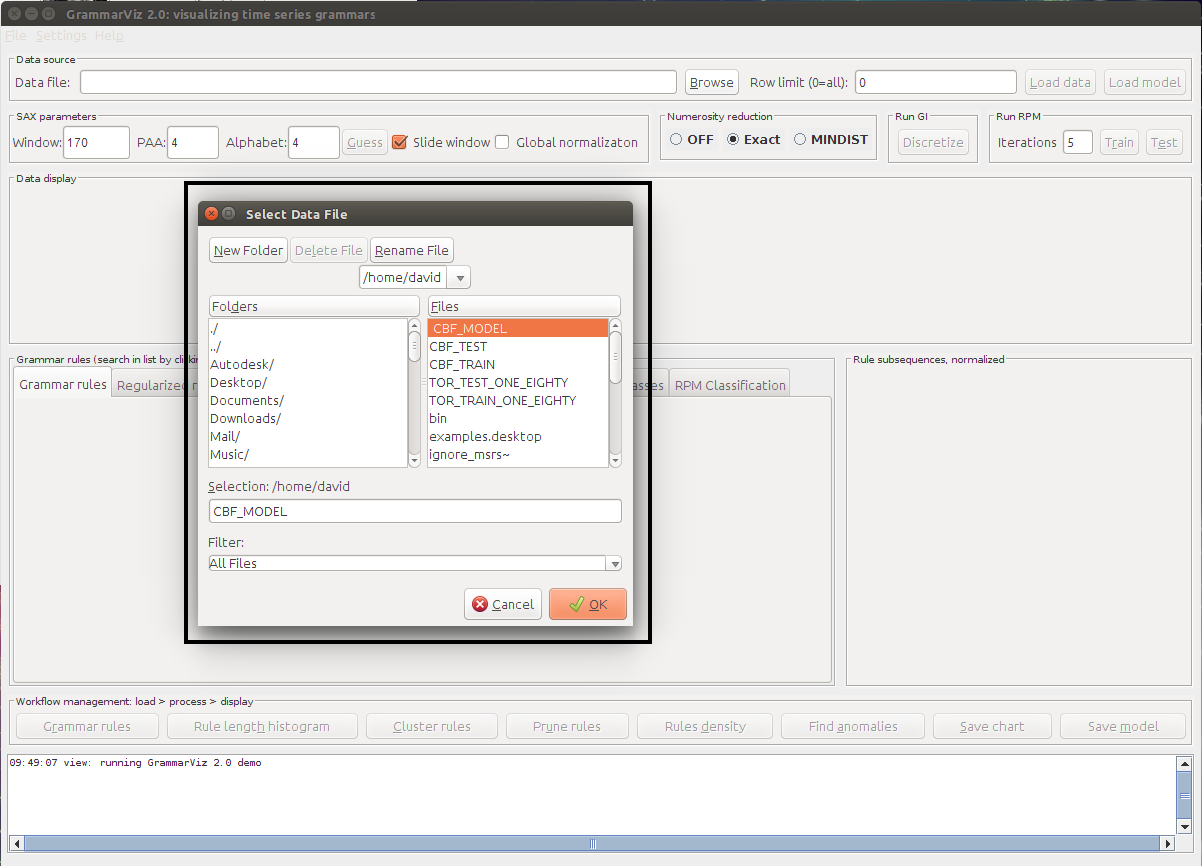
\includegraphics[width=\textwidth]{TSAT-load-model-step-2}
	\caption{Open the file browser prompt}
	\label{fig:TSAT-load-model-step-2}
\end{figure}

\newpage
\paragraph{Step 3}
Once the model has been selected, click the ``Load Model'' button and the model will be loaded into TSAT. If the data is not found during the loading step TSAT will ask for the location of the data using a file browser prompt, like in figure \ref{fig:TSAT-load-model-failed-data}, simple provide the data and the model will finish loading. 

\begin{figure}[H]
	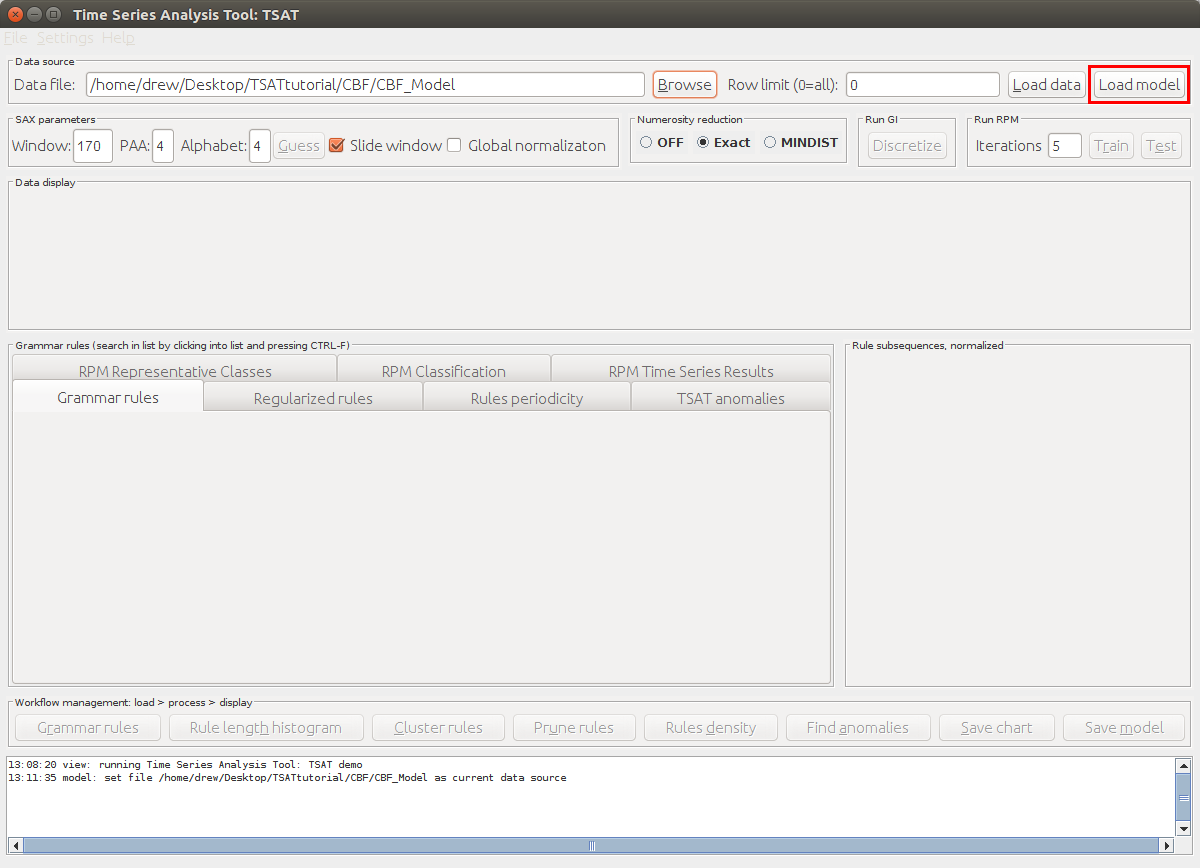
\includegraphics[width=\textwidth]{TSAT-load-model-step-3}
	\caption{Model loaded}
	\label{fig:TSAT-load-model-step-3}
\end{figure}

\begin{figure}[H]
	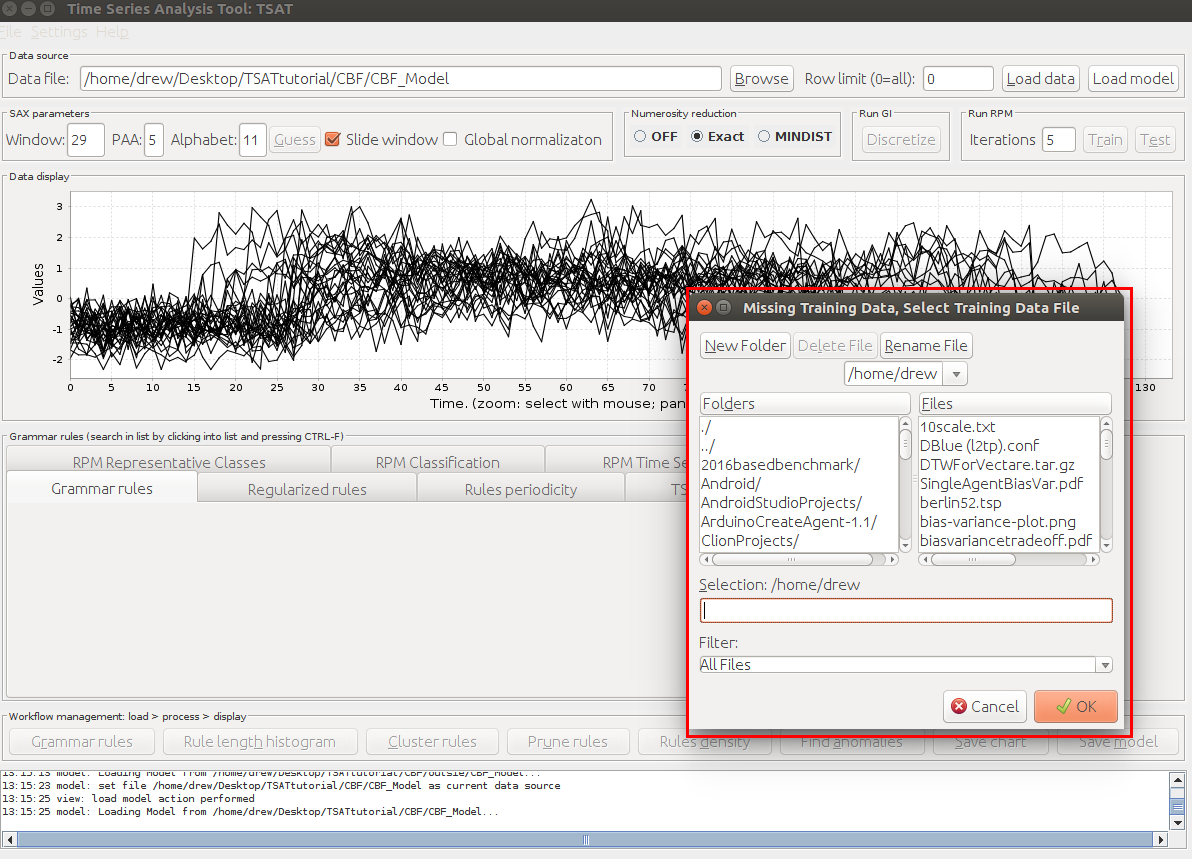
\includegraphics[width=\textwidth]{TSAT-load-model-failed-data}
	\caption{Missing training data file browser prompt}
	\label{fig:TSAT-load-model-failed-data}
\end{figure}

\subsection{Settings}
\label{RPMSettings}
There are a few options that can be changed when using RPM in TSAT, some of them have already been mentioned and will be covered again.

\subsubsection{Dynamic Time Warping}
\label{DTW}
Dynamic Time Warping, or DTW, is a method of measuring distance between two time series, this means how similar or different they are to each other. By default RPM uses Euclidean distance which is a simple and fast measurement, however it does not do well when the similar patterns between time series occur at different positions. This is where DTW comes in, it can handle temporal shifts in patterns and, depending on the data, can vastly improve the accuracy of the model. There is a cost however, DTW is a much slower operation and is very expensive to run so it is left as an option for the user. 

DTW also has another parameter called ``Window'' which can have dramatic effects on DTW both in how long it takes to run and its accuracy. The window size basically limits how far DTW will go to try to accurately try to match the two time series. A smaller window will stop DTW from trying to over match them and will take less time to compute. A larger window will take much longer to compute but can allow DTW to match patterns that are father apart. Choosing a good window size can be highly dependent on the data and what is being compared, and therefore some experimentation may be needed to find a good window size. There are a few good rules when choosing a window size, for one a window size greater then 10 will usually give bad results so 10 is considered a good starting point. Often for the more common types of data a 3-5 window size can be much better option with significant speed ups. Note DTW's window should not be confused with the Window size in the SAX parameters section of the main window, these are two different and distinct uses of the word window. 

\newpage
\paragraph{Step 1}
To change between Euclidean distance and DTW first open the settings menu:

``Settings''$\rightarrow$``TSAT options'' or press Ctrl+p. This will bring up the settings menu in figure \ref{fig:TSAT-settings-dialog}.

\begin{figure}[H]
	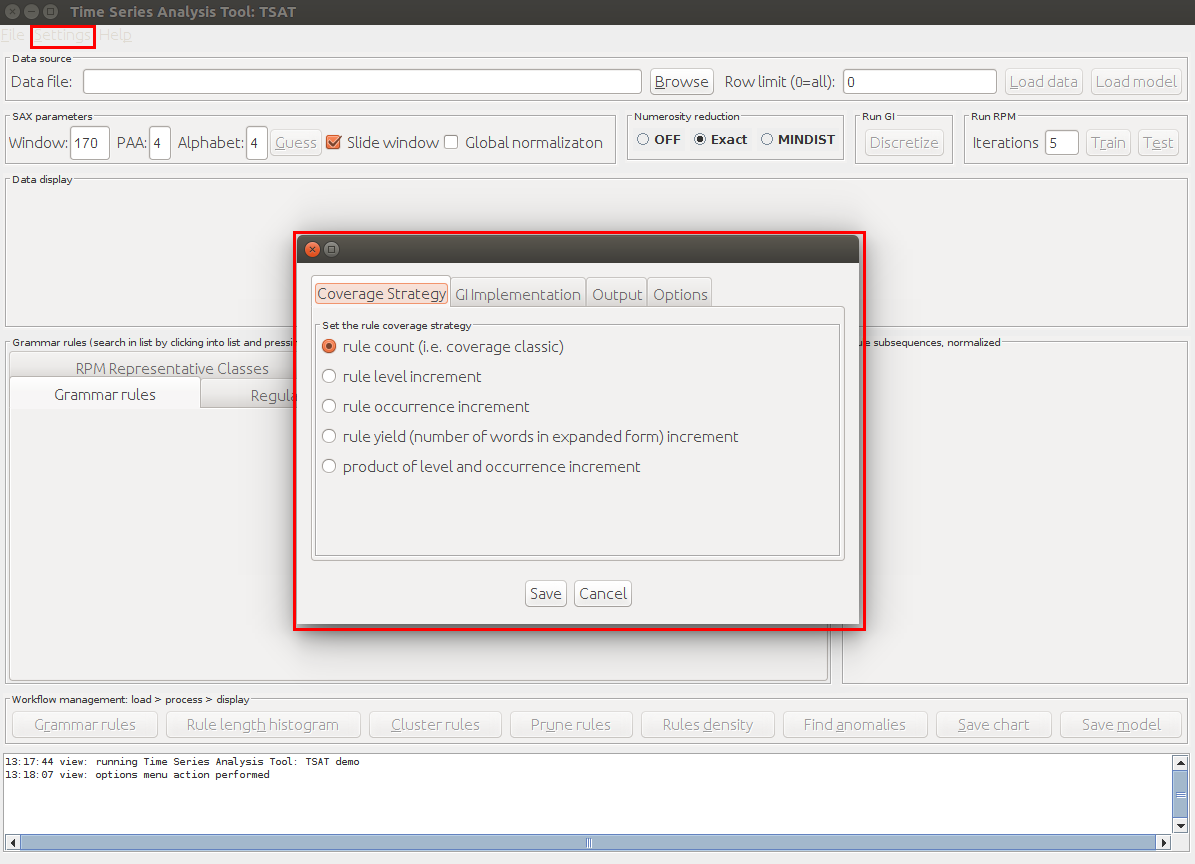
\includegraphics[width=\textwidth]{TSAT-settings-dialog}
	\caption{TSAT Settings Dialog}
	\label{fig:TSAT-settings-dialog}
\end{figure}

\newpage
\paragraph{Step 2}
Now click on the ``Options'' tab.

\begin{figure}[H]
	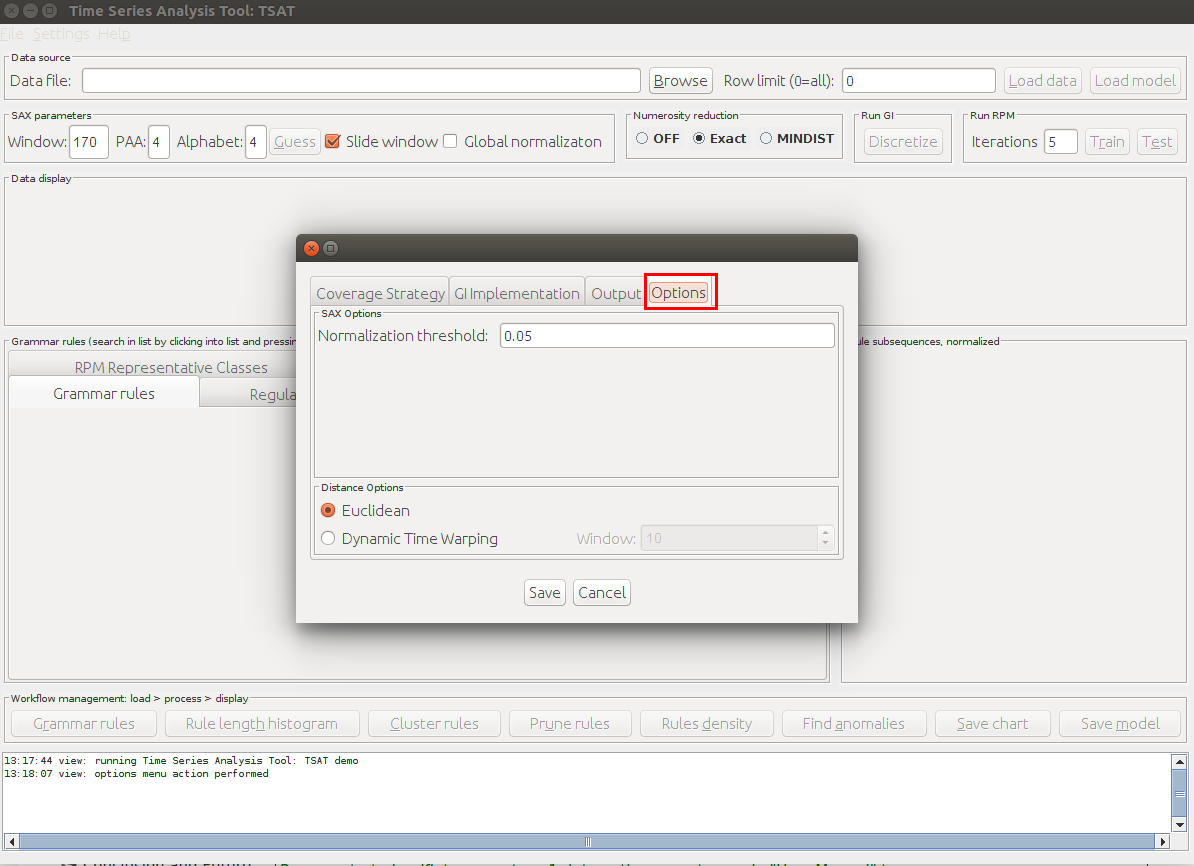
\includegraphics[width=\textwidth]{TSAT-settings-dialog-options}
	\caption{TSAT Settings Dialog Options}
	\label{fig:TSAT-settings-dialog-options}
\end{figure}

\newpage
\paragraph{Step 3}
Now select the ``Dynamic Time Warping'' option and the desired ``Window'' then click save.

\begin{figure}[H]
	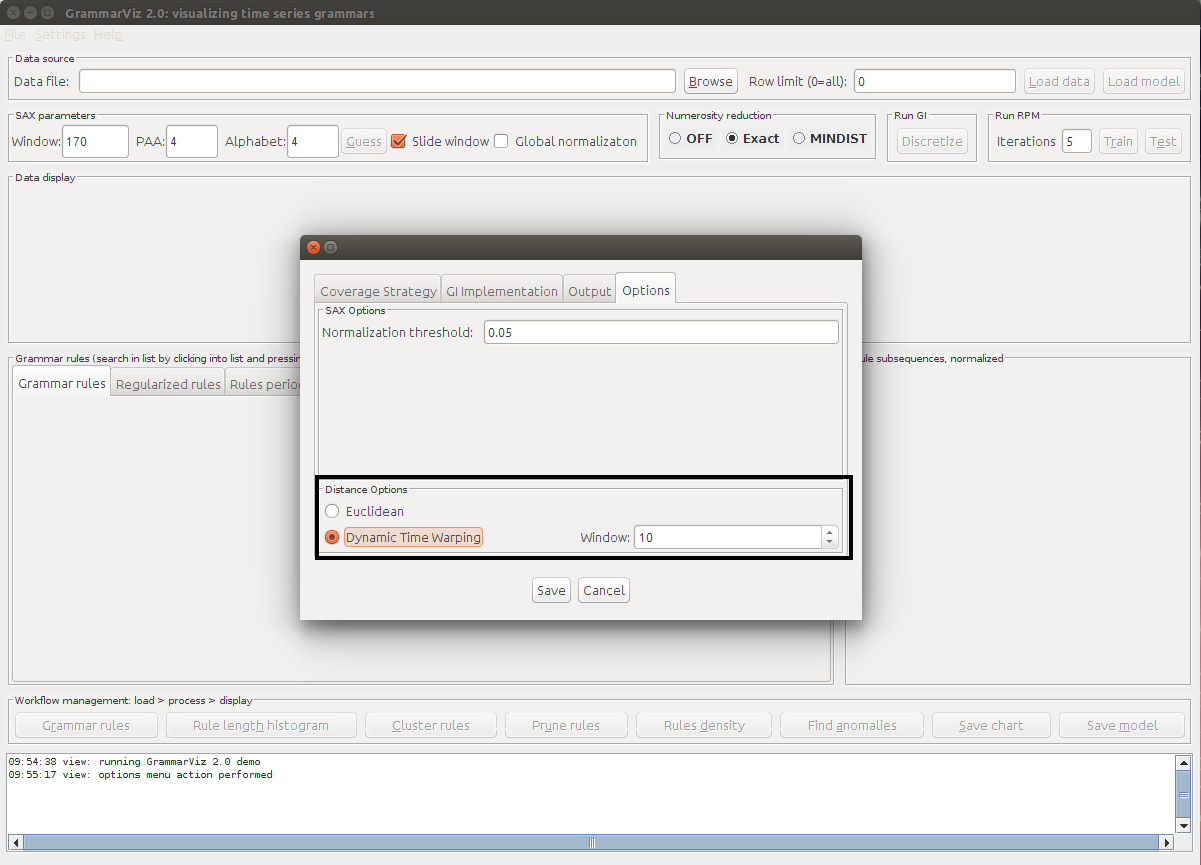
\includegraphics[width=\textwidth]{TSAT-settings-dialog-options-dtw}
	\caption{TSAT Settings Dialog Options DTW}
	\label{fig:TSAT-settings-dialog-options-dtw}
\end{figure}

\newpage
\subsubsection{Iterations}
\label{iterations}
During the operation of RPM it goes though a step that gets repeated many times. This step only stops under two conditions, a minimum threshold is met or if the maximum number of iterations are reached. The iterations setting found under the ``Run RPM'' section of the main window in TSAT is how the user can control the maximum number of iterations, figure \ref{fig:TSAT-iteration-setting}. The number of iterations can have an effect on how accurate the model can get, however the more iterations RPM runs through the longer it will take to complete. This becomes a balance between the quality of the model and the how long the training phase will take. It should also should be noted that RPM can stop before the maximum number of iterations is met if the model has reached an ideal state. However, this does not mean that all models will or even can reach an ideal state before the maximum number of iterations is reached, indeed some data sets may never return a model that meets the requirements. As RPM runs through the iterations the model should get better but the amount it gets better by can be come increasingly insignificant and therefore adding another 10 iterations may not add any significant results to the model. The only way to know if adding more iterations will improve the model is by experimentation which would involve training multiple times, increasing the maximum number of iterations every run until the testing results return no significant improvements.

\begin{figure}[H]
	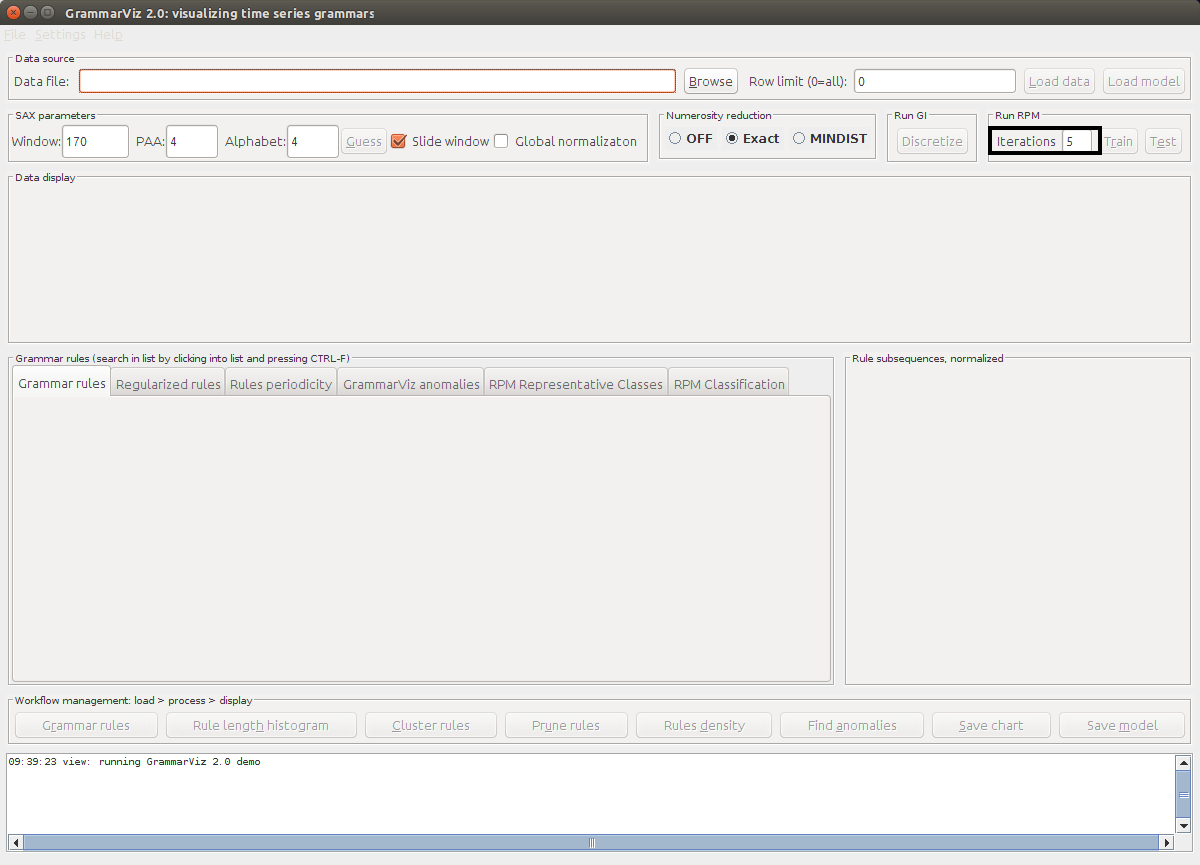
\includegraphics[width=\textwidth]{TSAT-iterations-setting}
	\caption{TSAT RPM Iteration Setting}
	\label{fig:TSAT-iteration-setting}
\end{figure}


\subsection{Python Interface}

There are three functions: RPMTrainTest, RPMTrain, and RPMTest and they can be called external from tsail.py as:

\begin{lstlisting}
tsail.RPMTrainTest(pathToTraining, pathToTest, outputFile, num_iters)
tsail.RPMTrain(pathToTraining, outputFile, num_iters)
tsail.RPMTest(pathToTest, modelFile, num_iters)
\end{lstlisting}

With parameters:
\begin{description}
	\item[pathToTraining] The path to the file containing the training time series data.
	\item[pathToTest] The path to the file containing the testing time series data.
	\item[outputFile] The name of the file that will be used for writing the returned json object and the serialized model file which can be used as input to RPMTest.
	\item[num\_iters] The number of RPM iterations to run.
	\item[modelFile]  The filename of the serialized model file.  Either saved from the GUI or generated by RPMTrainTest or RPMTrain.
\end{description}

For RPMTrainTest both training and testing will be output whereas in RPMTrain and RPMTest they each do exactly either training or testing. 

The training output is an array of:

\url{https://github.com/dwicke/TSAT/blob/72498ab66795e221eb6e26fbc65b0f156169ca66/src/main/java/edu/gmu/grammar/patterns/TSPattern.java}

TSPattern has the following properties that are accessible via the returned json object:

\begin{lstlisting}
private int frequency; // The number of times this pattern is used
private double[] patternTS; // the time series pattern
private double error = 0; // the pattern's error rate.
private String label; // The class label for the pattern
private int fromTS; // the index for the time series.
private int startP; // the patterns start position in the concatenated data.
\end{lstlisting}

The test output is a 2D array of strings for each instance we have the value corresponding to 
\texttt{[[\bsq{inst\#}, \bsq{actual class}, \bsq{predicted class}, \bsq{timeSeries}]]}

The test output when the data input is unlabeled is a 2D array of strings where for each instance we have:

\texttt{[[\bsq{inst\#}, \bsq{comma separated list of the probabilities of being in the particular class},\\\bsq{predicted class}, \bsq{timeSeries}]]}

When running RPMTrainTest you will generate three files as output instead of 1.

\texttt{<outputfileName>.train
<outputfileName>.test
<outputfileName>}

Files with the .train and .test extensions are the json of the python dictionaries as discussed in previous sections.  The last file can be imported into TSAT GUI as it is the same as the saved model in {\TSAT}. Example usage of all three functions are contained within tsail.py.

\section{FAQs}

When training there must always be more than one example from each class label and there must be more than one label.

\paragraph{Installation}

This tutorial assumes that you are running Ubuntu 16.04 with Java 1.8 or greater installed.

\begin{allintypewriter}
	\noindent git clone https://github.com/dwicke/TSAT.git\\
	cd TSAT\\
	mvn package -Psingle\\
\end{allintypewriter}
This will create tsat-0.0.1-SNAPSHOT-jar-with-dependencies.jar in the target directory.  You can execute the jar and run the GUI by double clicking on it after changing its permissions:
\begin{verbatim}
chmod +x tsat-0.0.1-SNAPSHOT-jar-with-dependencies.jar
\end{verbatim}  


To run the GUI from a shell you can do:
\begin{verbatim}
$ java -Xmx2g -jar target/tsat-0.0.1-SNAPSHOT-jar-with-dependencies.jar 
\end{verbatim}

The -Xmx2g allocates max of 2Gb of memory for the software.



\bibliographystyle{ieeetr}
\bibliography{citations}

\end{document}
